% Options for packages loaded elsewhere
\PassOptionsToPackage{unicode}{hyperref}
\PassOptionsToPackage{hyphens}{url}
\PassOptionsToPackage{dvipsnames,svgnames,x11names}{xcolor}
%
\documentclass[
  letterpaper,
  DIV=11,
  numbers=noendperiod]{scrartcl}

\usepackage{amsmath,amssymb}
\usepackage{iftex}
\ifPDFTeX
  \usepackage[T1]{fontenc}
  \usepackage[utf8]{inputenc}
  \usepackage{textcomp} % provide euro and other symbols
\else % if luatex or xetex
  \usepackage{unicode-math}
  \defaultfontfeatures{Scale=MatchLowercase}
  \defaultfontfeatures[\rmfamily]{Ligatures=TeX,Scale=1}
\fi
\usepackage{lmodern}
\ifPDFTeX\else  
    % xetex/luatex font selection
\fi
% Use upquote if available, for straight quotes in verbatim environments
\IfFileExists{upquote.sty}{\usepackage{upquote}}{}
\IfFileExists{microtype.sty}{% use microtype if available
  \usepackage[]{microtype}
  \UseMicrotypeSet[protrusion]{basicmath} % disable protrusion for tt fonts
}{}
\makeatletter
\@ifundefined{KOMAClassName}{% if non-KOMA class
  \IfFileExists{parskip.sty}{%
    \usepackage{parskip}
  }{% else
    \setlength{\parindent}{0pt}
    \setlength{\parskip}{6pt plus 2pt minus 1pt}}
}{% if KOMA class
  \KOMAoptions{parskip=half}}
\makeatother
\usepackage{xcolor}
\setlength{\emergencystretch}{3em} % prevent overfull lines
\setcounter{secnumdepth}{-\maxdimen} % remove section numbering
% Make \paragraph and \subparagraph free-standing
\ifx\paragraph\undefined\else
  \let\oldparagraph\paragraph
  \renewcommand{\paragraph}[1]{\oldparagraph{#1}\mbox{}}
\fi
\ifx\subparagraph\undefined\else
  \let\oldsubparagraph\subparagraph
  \renewcommand{\subparagraph}[1]{\oldsubparagraph{#1}\mbox{}}
\fi


\providecommand{\tightlist}{%
  \setlength{\itemsep}{0pt}\setlength{\parskip}{0pt}}\usepackage{longtable,booktabs,array}
\usepackage{calc} % for calculating minipage widths
% Correct order of tables after \paragraph or \subparagraph
\usepackage{etoolbox}
\makeatletter
\patchcmd\longtable{\par}{\if@noskipsec\mbox{}\fi\par}{}{}
\makeatother
% Allow footnotes in longtable head/foot
\IfFileExists{footnotehyper.sty}{\usepackage{footnotehyper}}{\usepackage{footnote}}
\makesavenoteenv{longtable}
\usepackage{graphicx}
\makeatletter
\def\maxwidth{\ifdim\Gin@nat@width>\linewidth\linewidth\else\Gin@nat@width\fi}
\def\maxheight{\ifdim\Gin@nat@height>\textheight\textheight\else\Gin@nat@height\fi}
\makeatother
% Scale images if necessary, so that they will not overflow the page
% margins by default, and it is still possible to overwrite the defaults
% using explicit options in \includegraphics[width, height, ...]{}
\setkeys{Gin}{width=\maxwidth,height=\maxheight,keepaspectratio}
% Set default figure placement to htbp
\makeatletter
\def\fps@figure{htbp}
\makeatother

\KOMAoption{captions}{tableheading}
\makeatletter
\@ifpackageloaded{tcolorbox}{}{\usepackage[skins,breakable]{tcolorbox}}
\@ifpackageloaded{fontawesome5}{}{\usepackage{fontawesome5}}
\definecolor{quarto-callout-color}{HTML}{909090}
\definecolor{quarto-callout-note-color}{HTML}{0758E5}
\definecolor{quarto-callout-important-color}{HTML}{CC1914}
\definecolor{quarto-callout-warning-color}{HTML}{EB9113}
\definecolor{quarto-callout-tip-color}{HTML}{00A047}
\definecolor{quarto-callout-caution-color}{HTML}{FC5300}
\definecolor{quarto-callout-color-frame}{HTML}{acacac}
\definecolor{quarto-callout-note-color-frame}{HTML}{4582ec}
\definecolor{quarto-callout-important-color-frame}{HTML}{d9534f}
\definecolor{quarto-callout-warning-color-frame}{HTML}{f0ad4e}
\definecolor{quarto-callout-tip-color-frame}{HTML}{02b875}
\definecolor{quarto-callout-caution-color-frame}{HTML}{fd7e14}
\makeatother
\makeatletter
\@ifpackageloaded{caption}{}{\usepackage{caption}}
\AtBeginDocument{%
\ifdefined\contentsname
  \renewcommand*\contentsname{Table of contents}
\else
  \newcommand\contentsname{Table of contents}
\fi
\ifdefined\listfigurename
  \renewcommand*\listfigurename{List of Figures}
\else
  \newcommand\listfigurename{List of Figures}
\fi
\ifdefined\listtablename
  \renewcommand*\listtablename{List of Tables}
\else
  \newcommand\listtablename{List of Tables}
\fi
\ifdefined\figurename
  \renewcommand*\figurename{Figure}
\else
  \newcommand\figurename{Figure}
\fi
\ifdefined\tablename
  \renewcommand*\tablename{Table}
\else
  \newcommand\tablename{Table}
\fi
}
\@ifpackageloaded{float}{}{\usepackage{float}}
\floatstyle{ruled}
\@ifundefined{c@chapter}{\newfloat{codelisting}{h}{lop}}{\newfloat{codelisting}{h}{lop}[chapter]}
\floatname{codelisting}{Listing}
\newcommand*\listoflistings{\listof{codelisting}{List of Listings}}
\makeatother
\makeatletter
\makeatother
\makeatletter
\@ifpackageloaded{caption}{}{\usepackage{caption}}
\@ifpackageloaded{subcaption}{}{\usepackage{subcaption}}
\makeatother
\ifLuaTeX
  \usepackage{selnolig}  % disable illegal ligatures
\fi
\usepackage{bookmark}

\IfFileExists{xurl.sty}{\usepackage{xurl}}{} % add URL line breaks if available
\urlstyle{same} % disable monospaced font for URLs
\hypersetup{
  pdftitle={Analyzing School District Data for Improvement},
  pdfauthor={Dan Swart; SCUC-ISD Board of Trustees; Seat 6},
  colorlinks=true,
  linkcolor={blue},
  filecolor={Maroon},
  citecolor={Blue},
  urlcolor={Blue},
  pdfcreator={LaTeX via pandoc}}

\title{Analyzing School District Data for Improvement}
\usepackage{etoolbox}
\makeatletter
\providecommand{\subtitle}[1]{% add subtitle to \maketitle
  \apptocmd{\@title}{\par {\large #1 \par}}{}{}
}
\makeatother
\subtitle{\textbf{\emph{The Power of QUARTO}}}
\author{Dan Swart \and SCUC-ISD Board of Trustees \and Seat 6}
\date{2024-02-28}

\begin{document}
\maketitle

\Large

\begin{tcolorbox}[enhanced jigsaw, leftrule=.75mm, breakable, bottomrule=.15mm, opacityback=0, colframe=quarto-callout-tip-color-frame, arc=.35mm, colback=white, rightrule=.15mm, left=2mm, toprule=.15mm]

``My aim here is to contribute something to the improvement of learning
in our school district; or any school district. My goal is to build a
collabrative community in the education domain helping each other find
better and better ways of using data to guide, improve and govern their
systems of learning.

I look forward to the day when everyone at every level is comfortable
sketching a simple flow diagram, trying some changes, and plotting the
results to see if the changes worked. This straightforward process makes
possible and encourages the study of different methods of learning and
administration (inputs) and their impact on the results observed
(outputs) \textbf{\emph{at the local level.}} Those interested in using
data to help improve learning in their district please feel free to
contact me.'' \bigskip

-- Dan Swart

\end{tcolorbox}

\vspace{0.3in}

\section{\texorpdfstring{\textbf{INTRODUCTION}}{INTRODUCTION}}\label{introduction}

Everyone at every level in a school district is trying to answer
important, practical questions and seek data to help them. Those
questions include:

\begin{itemize}
\item
  The numbers vary from time period to time period. \textbf{Does that
  variation signal anything important?}
\item
  Is the variation I see due to normal \textbf{random fluctuations} that
  are present in all measurements, or to some strong influence(s) now
  present in the system?
\item
  Do the varying numbers \textbf{constitute a trend} (good, or bad)?
\item
  What is the \textbf{demonstrated output capability} of our district to
  deliver STAAR scores (or any other results) in the various categories
  and levels? In other words, what is \textbf{rational} to expect from
  our system \textbf{in the future?}
\item
  \textbf{Should we continue} a particular approach, \textbf{abandon}
  it, or \textbf{continue it with modification?}
\item
  Should we change something right away with an intervention, \textbf{or
  will that make things worse?}
\item
  Under current leadership, are we improving, staying the same, or
  getting worse, and \textbf{how can we tell?}
\end{itemize}

\textbf{\emph{If you are a board member, district employee, or concerned
citizen who asks themselves questions like these, this paper can help
you. If you find little value in changing how you use data as a guide
for action, this paper is definitely not for you.}}

This paper is for anyone striving to improve learning in their school
district and who think data can help them. Anyone can use the simple
theory and techniques to significantly improve their teaching,
classrooms, campuses, departments and districts.

To improve our systems of learning in a rational, systematic way we need
new information beyond that supplied by merely `description-only'
reports. Only a few simple changes are required.

Currently, neither the Texas Education Agency (TEA) nor the Texas
Association of School Boards (TASB) offer training or support in the
appropriate methods and tools that would give school boards and
administrators access to the new information they need.

I predict that educators who learn to draw a very simple flow diagram
and very simple charts can (and will) improve any results they wish to
improve. These simple tools allow anyone to examine how the inputs of a
learning process may (or may not) affect the outputs of the process.
Although they are prettier coming from a computer, they can, quite
literally, be constructed with a piece of newsprint and a crayon.

Thus, anyone can experiment on a small scale and evaluate the results
before attempting large scale changes. Those results are easily shared
with others, such as school boards and administrators, and form a
rational basis for understanding the results observed and any proposed
changes.

All that is required is an open mind, willingness to do things a little
differently, and a sense of urgency for getting things done. That sounds
like Texans, to me.

\vspace{0.3in}

\section{\texorpdfstring{\textbf{BACKGROUND}}{BACKGROUND}}\label{background}

All school boards and superintendents work very hard to `keep the lights
on' and improve learning in their districts and campuses (or `campi' if
you prefer the Latin form, because it \textbf{\emph{is}} funnier).

Administration of budgets for facilities, equipment, personnel, safety
and legislative compliance is a function of the managerial skill of the
executive team and the school board. It is usually well managed with
thoughtful planning and careful attention to fiscal details. Both TEA
and TASB supply quality education and support for the budgeting element
of school board responsibility.

Improving learning in a district is a very different challenge and
requires a different set of skills and knowledge.

Currently, there are dozens of situations where we need better ways to
evaluate our data.

\begin{longtable}[]{@{}ll@{}}
\caption{{\textbf{Here are just a few examples of data that come our
way:}}}\tabularnewline
\toprule\noalign{}
Example Metric & Example Metric \\
\midrule\noalign{}
\endfirsthead
\toprule\noalign{}
Example Metric & Example Metric \\
\midrule\noalign{}
\endhead
\bottomrule\noalign{}
\endlastfoot
STAAR scores & Survey results \\
District improvement plans & TAPR reports \\
Dropout rates & Pedagogy review \\
On-time arrivals for buses & Attendance rates \\
Superintendent evaluations & Graduation rates \\
Superintendent searches & Accountability ratings \\
\end{longtable}

To make better decisions, the \textbf{\emph{`description-only'}} reports
we currently use to evaluate the performance of programs, pedagogy,
people, or anything else must come to us in a slightly different format
than what we are used to seeing.

Any evaluation of results must go beyond what is included in `snapshot'
reports, or even reports with two-point or three-point comparisons. As
discussed later, trends cannot be established with only two or three
data points.

As it turns out, the ``new'' information we need is already there in our
data, but it is `hidden'. As long as we continue to use and rely on
\textbf{\emph{`description-only'}} reports this critical information
\textbf{\emph{will remain hidden from us.}}

The following report is called an \textbf{\emph{Individuals Chart (part
of an XmR chart pair)}}\footnote{The chart shown is the `Individuals'
  chart. A complete XmR chart presentation also includes the `Moving
  Range' chart that plots the size of the up-and-down movement between
  data points. The Moving Range chart is used to calculate the range of
  values that is considered `normal' for the process (i.e., the `common
  cause' variation present in the process).} \footnote{The `XmR' chart
  is one of a family of `control charts' invented and developed by
  Walter A. Shewhart in 1929 while an engineer at Bell Telephone
  Laboratories. They are still the gold standard tool for understanding
  a process by separating `common cause' variation from `special cause'
  variation. The XmR chart is the ``voice of the process'' and reveals
  if your process is stable (predictable) or subject to a strong
  influence that makes it unpredictable.} and it is an example of what a
report looks like that includes the information necessary to create
well-codified reports, charts, and documents that are concise and
reliable. This chart analyzes public STAAR data provided by TEA, and
includes a brief interpretation of the chart. The XmR chart provides a
baseline (context) for evaluating both past and future performance.

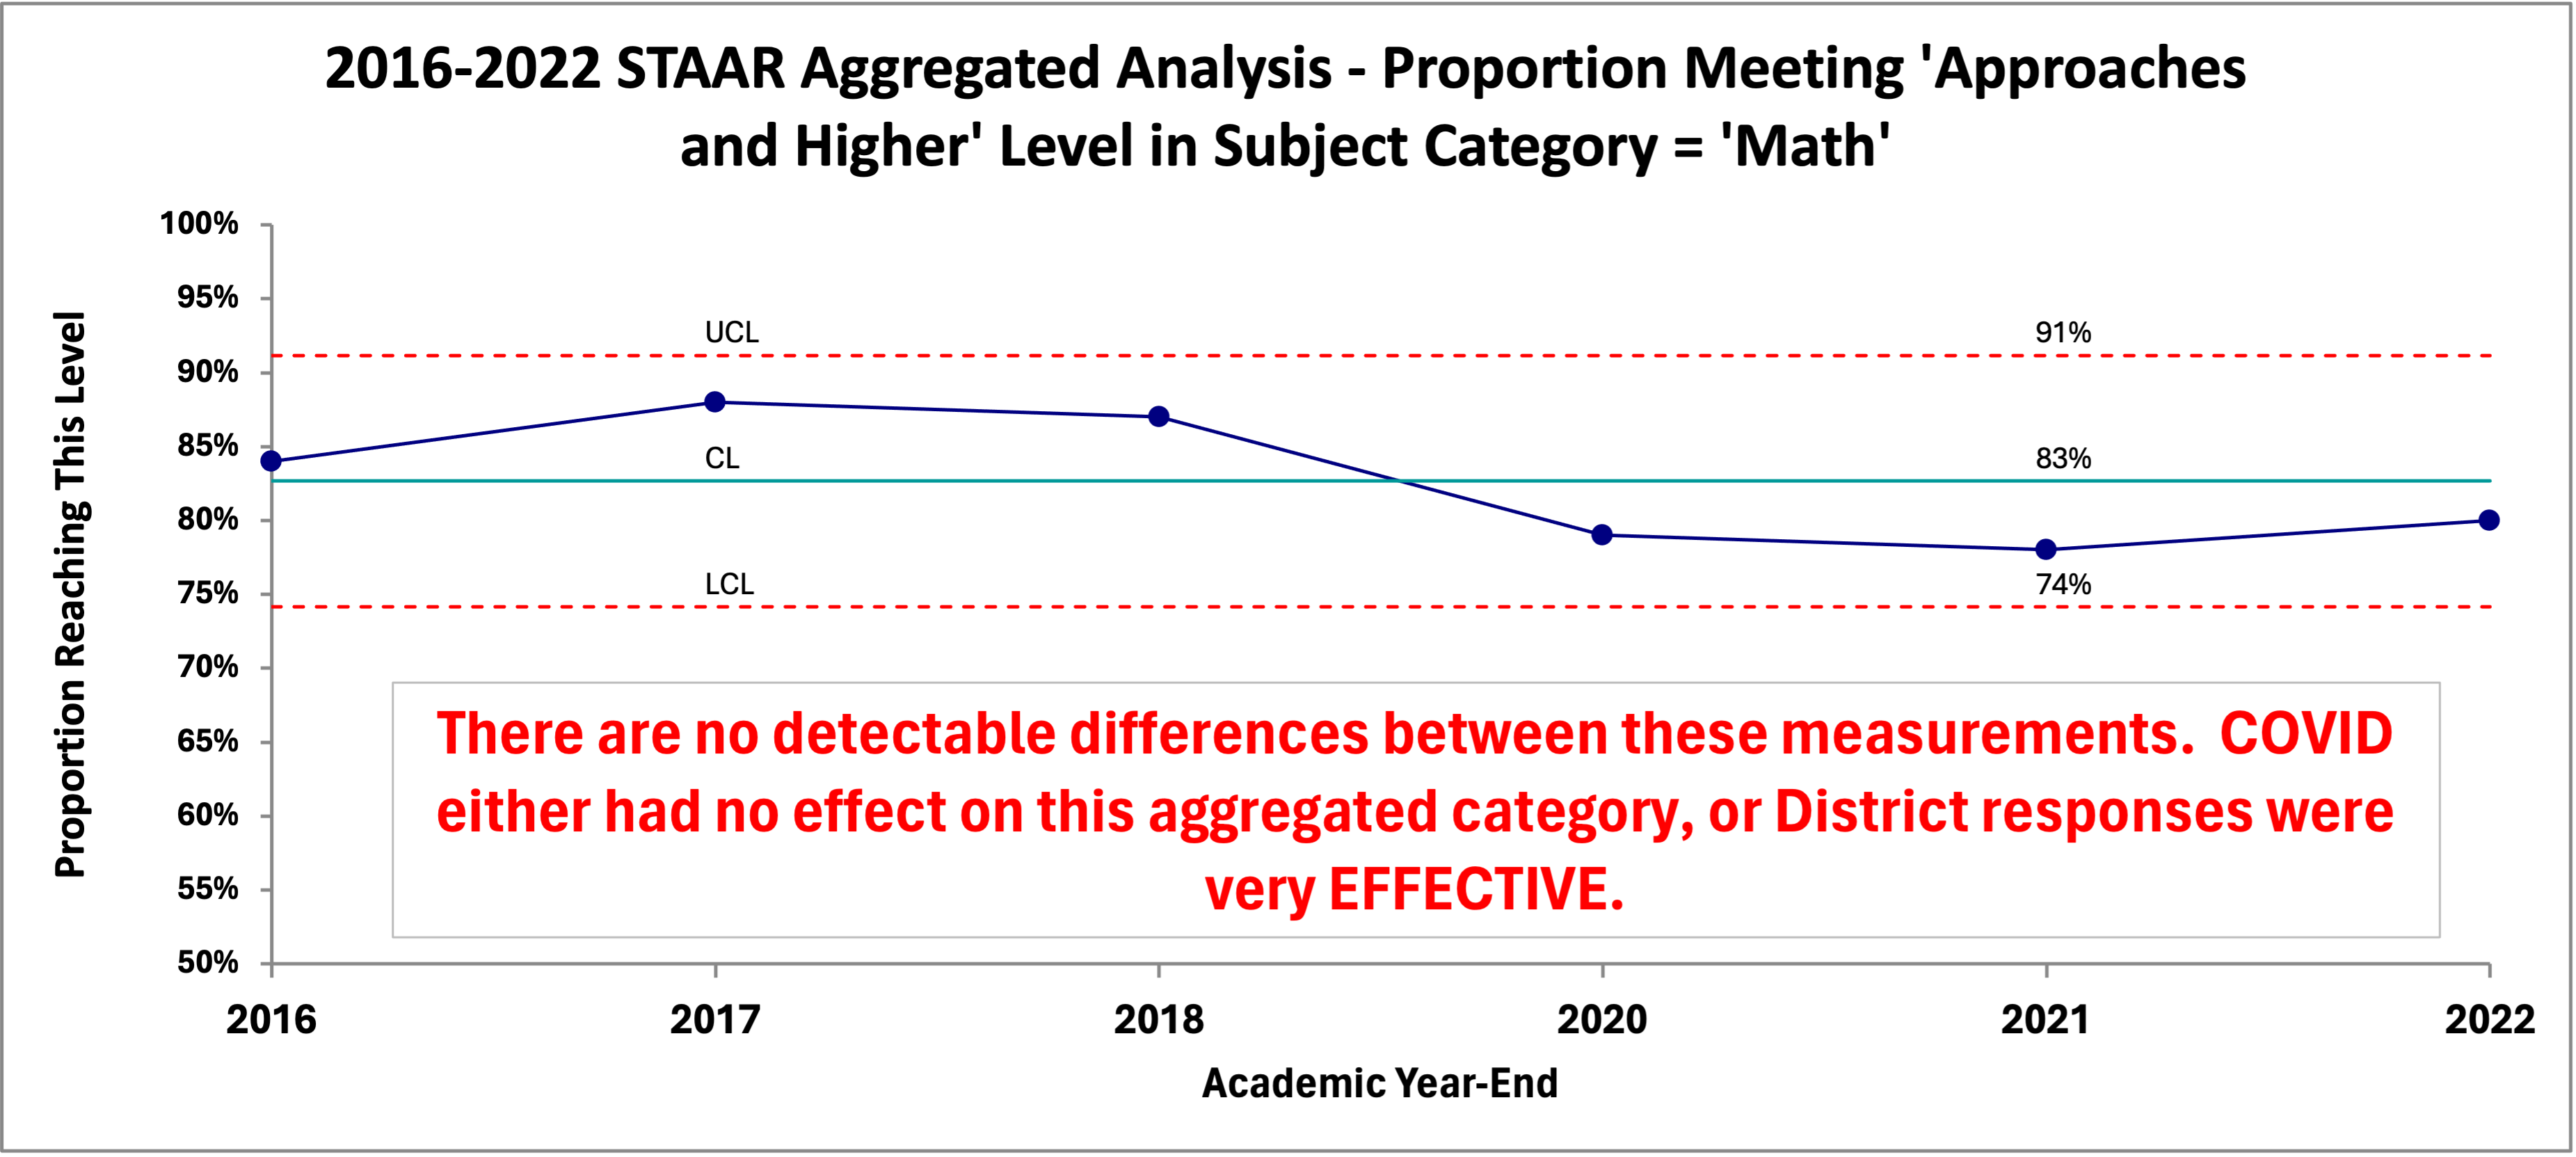
\includegraphics{pbc/xmr-2016-2022-math-approaches-combo.png} Fig: Data
taken from 5 TEA ``Snapshot'' description-only reports and 1 TAPR
description-only report

\vspace{0.3in}

\subsection[INTERPRETING THE CHART]{\texorpdfstring{INTERPRETING THE
CHART\footnote{Since interpretation of the chart concerns
  \textbf{\emph{future}} results expected of the process, the chart
  represents evidence that should influence our degree of belief in what
  the future holds. Since the future is uncertain, there is always some
  probability that our expectation will be wrong. Additional data helps
  a lot to reduce the uncertainty but will never eliminate it.}}{INTERPRETING THE CHART}}\label{interpreting-the-chart3}

\begin{itemize}
\item
  The measurements (the outputs) do go up and down, but
  \textbf{\emph{there is no numerical evidence that the movements are
  more than random variation}}. The ups and downs are almost certainly
  due to the many random forces acting on the cause system that produced
  the results (the inputs). This is called \textbf{\emph{common cause
  variation}} because the forces acting on the system are common to all
  the results we see.
\item
  In this case, the chart shows that all measurements fall between the
  calculated Upper Limit (UCL) and Lower Limit (LCL), with no
  statistical trends\footnote{Statistical techniques to detect `trends'
    exist and require 7 or more data points to detect. A special `trend'
    occurs when a point falls outside the range of `normal' variation.
    This is called a `special' cause of variation. The rules to detect
    these trends are easily learned and are built in to software that
    specializes in control chart preparation.} identified. Accordingly,
  the process is \textbf{\emph{stable}}, with a
  \textbf{\emph{predictable output capability}}. Of the many forces
  influencing the results, no one of them is predominant. If one force
  (or a small combination of forces) was predominate the chart would
  reveal it.
\end{itemize}

\begin{itemize}
\item
  If the process remains fundamentally the same, \textbf{the proportion
  of students in the district taking the STAAR exam in Math that reach
  the level of `Approaches Grade Level Standard, or Higher' will
  continue to fluctuate between 91\% and 74\%, with an average
  proportion of 81\% (the CL)}.
\item
  Given the data in the chart, any expectation of results outside those
  limits, without a significant change to the system,
  \textbf{\emph{would not be justified - at all}} (even if that
  expectation comes from the legislature and the TEA in the form of
  revised scoring criteria).
\item
  Any future result, if it falls inside the calculated boundaries
  \textbf{\emph{does not signify an increase or decrease in the
  performance of the process.}} Understanding this rule prevents
  `over-reacting' to random fluctuations. Every `up' or `down' does not
  mean we are doing better, or worse.
\item
  Confidence in the interpretation will \textbf{increase} as you add
  more data to the chart. For example, it would be helpful to add years
  prior to 2016 to see if our interpretation of the data changed.
\item
  This one chart includes all the information this data can reveal.
  \textbf{\emph{If you need or want more information you have to collect
  more data}}.
\end{itemize}

\begin{tcolorbox}[enhanced jigsaw, leftrule=.75mm, breakable, opacityback=0, toptitle=1mm, coltitle=black, opacitybacktitle=0.6, bottomrule=.15mm, colbacktitle=quarto-callout-important-color!10!white, colframe=quarto-callout-important-color-frame, arc=.35mm, bottomtitle=1mm, titlerule=0mm, title=\textcolor{quarto-callout-important-color}{\faExclamation}\hspace{0.5em}{Important}, colback=white, rightrule=.15mm, left=2mm, toprule=.15mm]

{\textbf{\emph{With this one simple chart}} we are in a position to
address each of the practical, important questions outlined earlier, at
least for this particular STAAR category and level. Why would you settle
for less? No other report even comes close.}

\end{tcolorbox}

\begin{tcolorbox}[enhanced jigsaw, leftrule=.75mm, breakable, opacityback=0, toptitle=1mm, coltitle=black, opacitybacktitle=0.6, bottomrule=.15mm, colbacktitle=quarto-callout-tip-color!10!white, colframe=quarto-callout-tip-color-frame, arc=.35mm, bottomtitle=1mm, titlerule=0mm, title=\textcolor{quarto-callout-tip-color}{\faLightbulb}\hspace{0.5em}{Interesting Observation:}, colback=white, rightrule=.15mm, left=2mm, toprule=.15mm]

{Following the COVID pandemic we all heard about the loss-of-learning
``crises'' in schools. I wanted to see if such a ``crises'' could be
detected using quantitative methods; not just personal opinion. The
quantitative evidence of the XmR chart indicates that even the extreme
government measures imposed during the COVID-19 pandemic apparently were
not disruptive enough to the district to create even a single point
outside the ``normal'' limits. Or, the counter-measures employed by the
district were very effective.}

\end{tcolorbox}

\vspace{0.3in}

\section{\texorpdfstring{\textbf{WHAT'S WRONG WITH THE
`DESCRIPTION-ONLY' REPORTS WE USE
NOW?}}{WHAT'S WRONG WITH THE `DESCRIPTION-ONLY' REPORTS WE USE NOW?}}\label{whats-wrong-with-the-description-only-reports-we-use-now}

The aim of a TEA report is `description-only'. \textbf{\emph{How many or
how much.}} They are estimates of how many people belong to this or that
category for a specified academic year. Or, to report the financial
aspects of operations during the school year. Their aim is \textbf{NOT}
to find out \textbf{WHY} there are so many or so few in this or that
category: merely how many.

The action to be taken is on the district, campus, or people studied. It
is a process designed for handing out reward and punishment.

On the other hand, school boards want to \textbf{\emph{improve learning
in the future.}}

Interest centers on future learning, not the learning of the past. For
example: adopt Policy B over A, or hold on to Policy A, or try Policy C
on a small scale (with further study).

The TEA collects data from every school in Texas, performs a multitude
of calculations, and produces reams of
\textbf{\emph{`description-only'}} reports and tables summarizing their
results by academic year. These \textbf{\emph{`description-only'}}
reports consist primarily of calculations mandated by the state
legislature, including those designed to allow districts to fulfill
their public notification requirements.

These statistical summaries are available to the public and the school
districts. Unfortunately, for the public and the school districts, the
information is not nearly as helpful as it could be. In fact, it takes
so much `data wrangling' to put it into a form that is remotely helpful
for assessing and improving district and campus learning that it is
simply not done.

Instead, administrators and school boards stare at endless rows and
columns of mind-numbing data fragments that are `sliced and diced' to an
extent that even
\href{https://en.wikipedia.org/wiki/Ron_Popeil}{\textcolor{blue}{\url{Ron  Popeil}}}
the inventor of the Chop-O-Matic would be envious!

After earnestly pouring over such \textbf{\emph{`description-only'}}
reports users still have no rational basis to predict what results to
expect in the future.

Here's a partial example from a \textbf{\emph{`description-only'}} TEA
report called a `Snapshot':

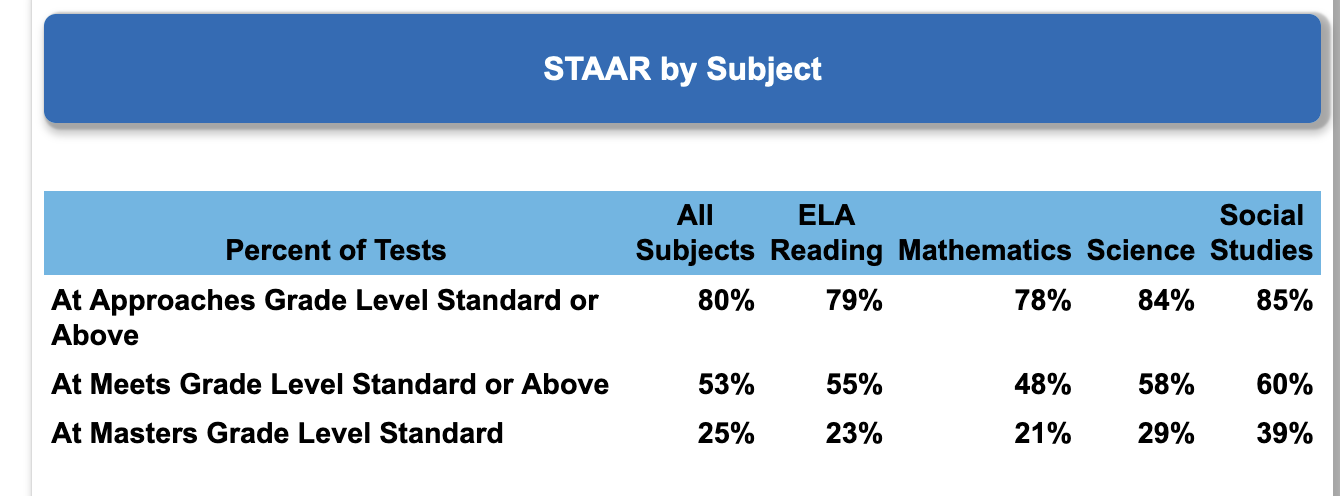
\includegraphics{img/staar-snapshot-example-2021-2022.png} Fig: Small
sample from TEAs Snapshot descrption-only report

The entire report can be found here:\\
\href{https://rptsvr1.tea.texas.gov/cgi/sas/broker?_service=marykay&_program=perfrept.perfmast.sas&_debug=0&ccyy=2022&lev=D&id=094902&prgopt=reports\%2Fsnapshot\%2Fsnapshot.sas}{\textcolor{blue}{\url{PDF Link}}}

(HTML Link)

And, here's a partial example from a TEA
\textbf{\emph{`description-only'}} report called a `School Report Card':

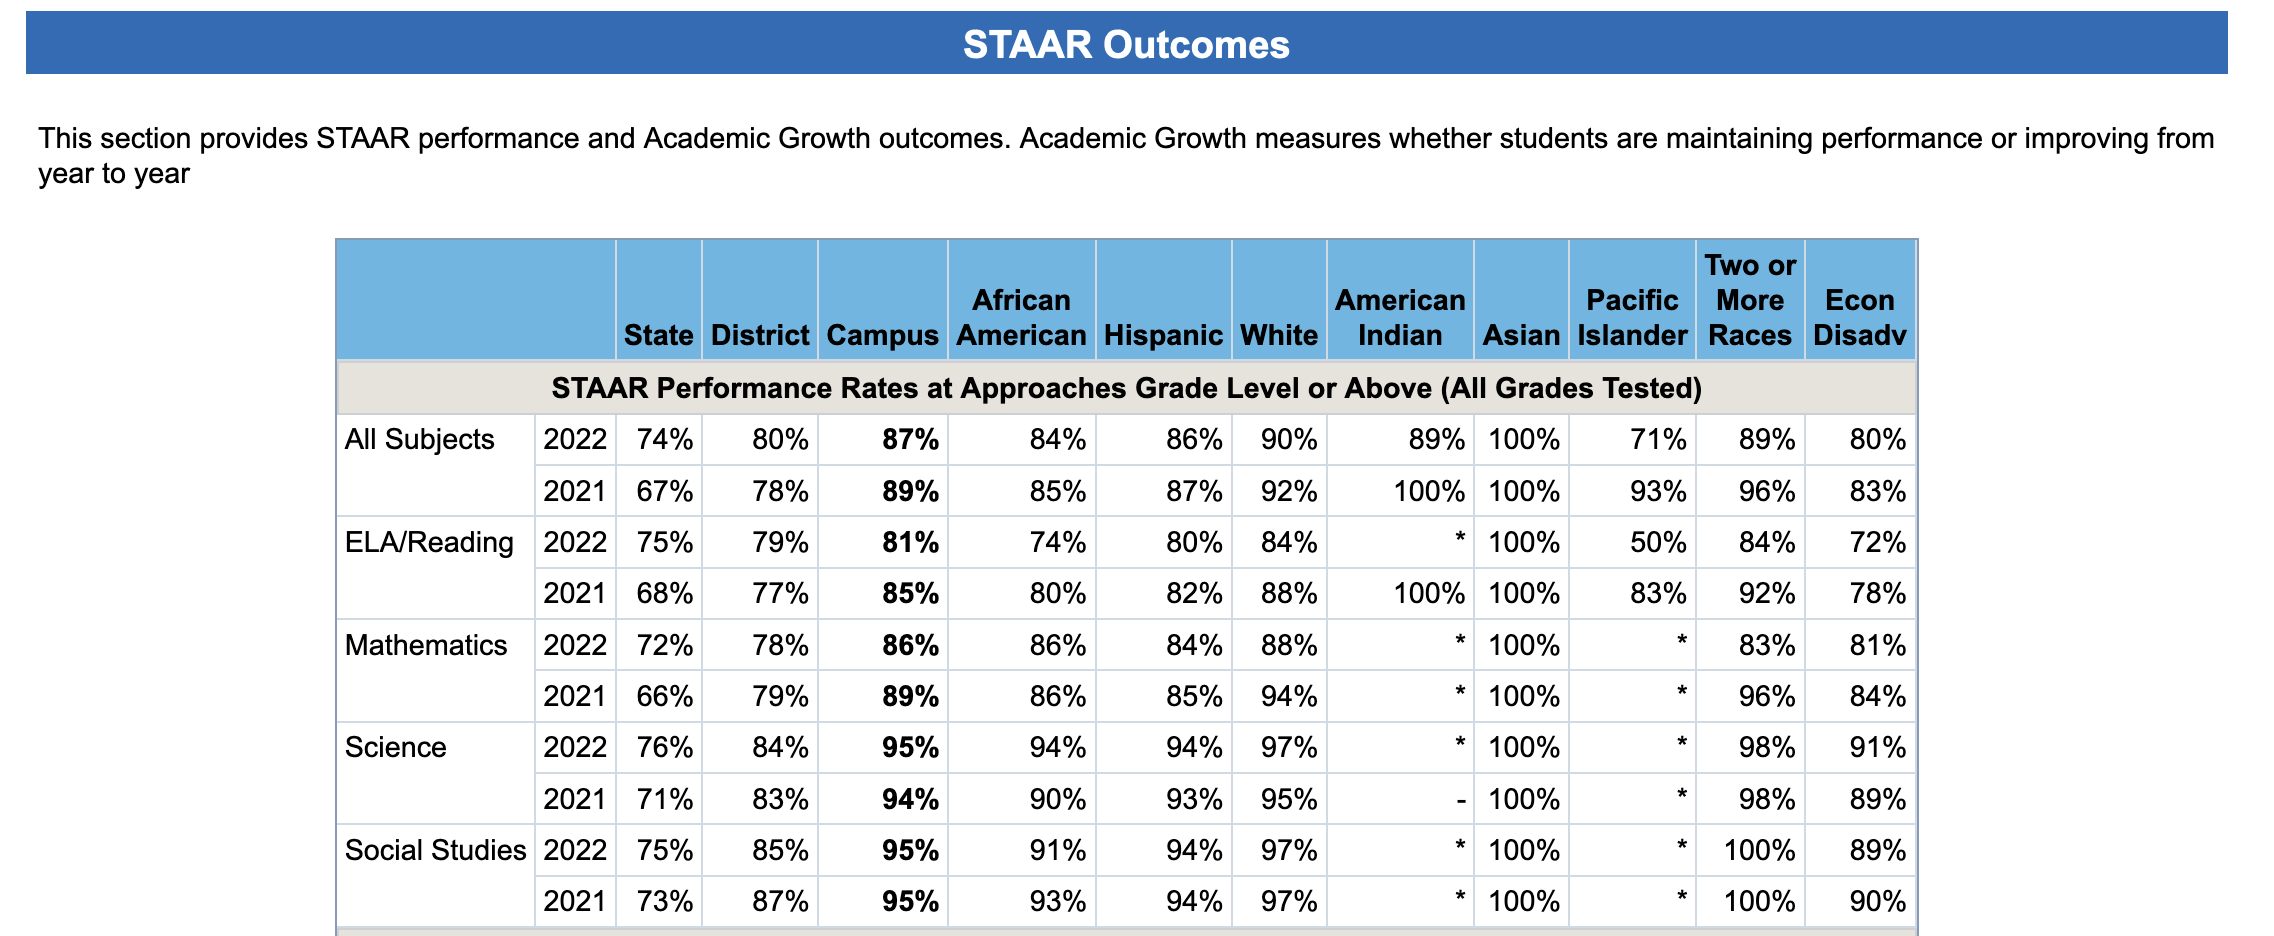
\includegraphics{img/staar-report-card-example-2021-2022.png}

Fig: Small sample from TEAs School Report Card description-only report

The entire report can be found here:\\
\href{https://rptsvr1.tea.texas.gov/cgi/sas/broker?_service=marykay&_program=perfrept.perfmast.sas&_debug=0&ccyy=2022&lev=C&prgopt=reports/src/src.sas&id=094902003}{\textcolor{blue}{\url{PDF Link}}}

(HTML Link)

\vspace{0.3in}

\section{\texorpdfstring{\textbf{OBSTACLES TO
IMPROVEMENT}}{OBSTACLES TO IMPROVEMENT}}\label{obstacles-to-improvement}

So, what is a school district to make of all these mountains of numbers
grouped and mixed together? Do they help districts improve learning in
the future? In their present form, the answer is definitely ``NO!''\\

\subsection{\texorpdfstring{\textbf{OBSTACLE
\#1}}{OBSTACLE \#1}}\label{obstacle-1}

When it comes to improving the system of education in a district this
`snapshot' view of the data has several very important limitations. One
is the grouping of several categories that probably represent different
processes into one group. Some TEA \textbf{\emph{`description-only'}}
reports combine more than one rating level into a single reporting
level. This assumes that the process that produced the results in one
category produces the results in them all.

For instance, one combines the `Approaches Grade Level' AND the `Meets
Grade Level' AND the `Masters Grade Level' ratings all into one combined
group total and calls it the ``Approaches Grade Level Standard AND
HIGHER'' level.

To make that category useful for improvement efforts we have to break it
into the three separate levels, so each represents a single situation
(process). Currently, that turns out to be quite tedious and extremely
time-consuming.

The `Snapshot' \textbf{\emph{`description-only'}} report offered by the
TEA is a good example. My hat is off to their programmers. It is an
impressive compilation of statistics all in one place. It is well-suited
for the needs of the TEA and their reporting responsibilities to the
legislature; but completely ill-suited for helping the concerned school
board, superintendent, or even tax-paying citizen make an analysis aimed
at improving future learning. One might call it a triumph of computation
over value.\\

Although this grouping of categories permits TEA to render abstract
judgments about a district or campus, the lack of specificity renders
these \textbf{\emph{`description-only'}} reports unsuitable for
understanding any particular process, category or level your board may
be interested in monitoring or improving. (Be mindful that this is not
TEA's fault; they must follow the direction of the legislative intent.)

\begin{tcolorbox}[enhanced jigsaw, leftrule=.75mm, breakable, opacityback=0, toptitle=1mm, coltitle=black, opacitybacktitle=0.6, bottomrule=.15mm, colbacktitle=quarto-callout-tip-color!10!white, colframe=quarto-callout-tip-color-frame, arc=.35mm, bottomtitle=1mm, titlerule=0mm, title=\textcolor{quarto-callout-tip-color}{\faLightbulb}\hspace{0.5em}{{It's like\ldots{}}}, colback=white, rightrule=.15mm, left=2mm, toprule=.15mm]

{trying to repair your car by reading the overall repair records of
similar models. What you need is diagnostic data about what is happening
(or not happening) with your \textbf{\emph{specific vehicle.}}}

\end{tcolorbox}

\vspace{0.3in}

Here is an example of several STAAR categories grouped together in a TEA
\textbf{\emph{`description-only'}} report:

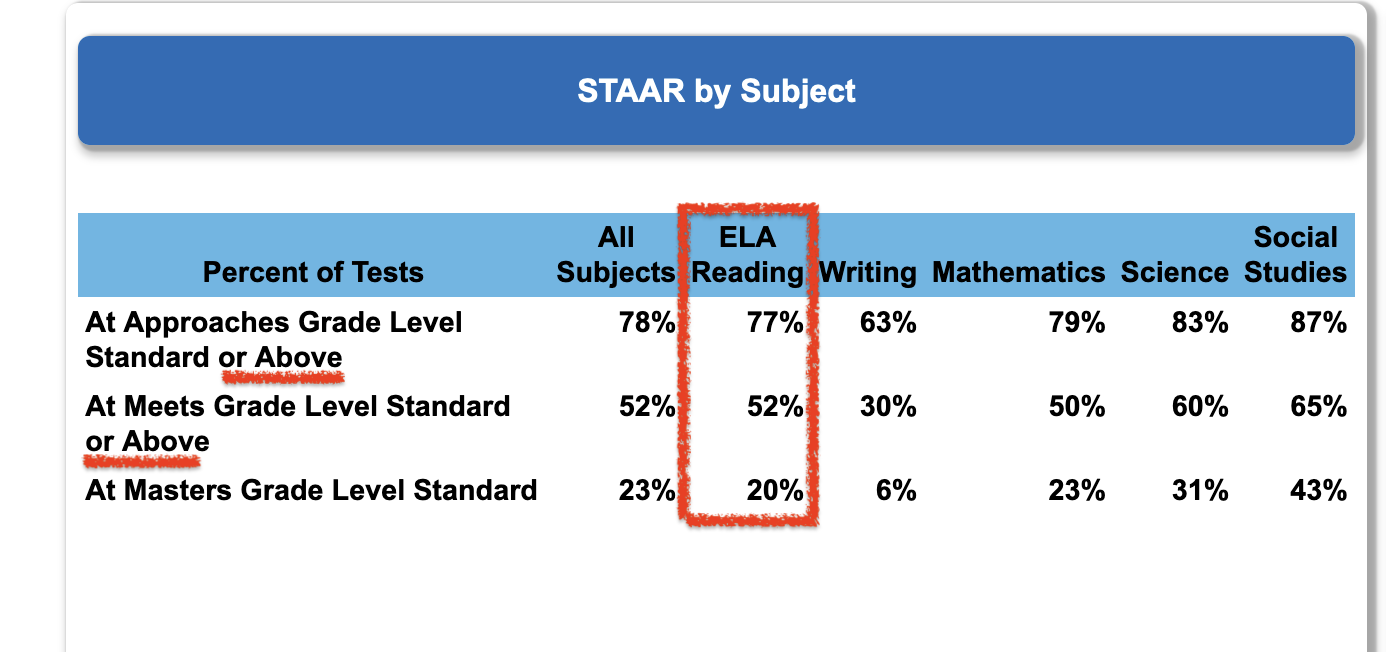
\includegraphics{img/staar-snapshot-by-subj-2022-2023-annot.png}

Fig: The first two rows combine more than one achievement level

Here's the section reporting STAAR scoring by ethnicity:

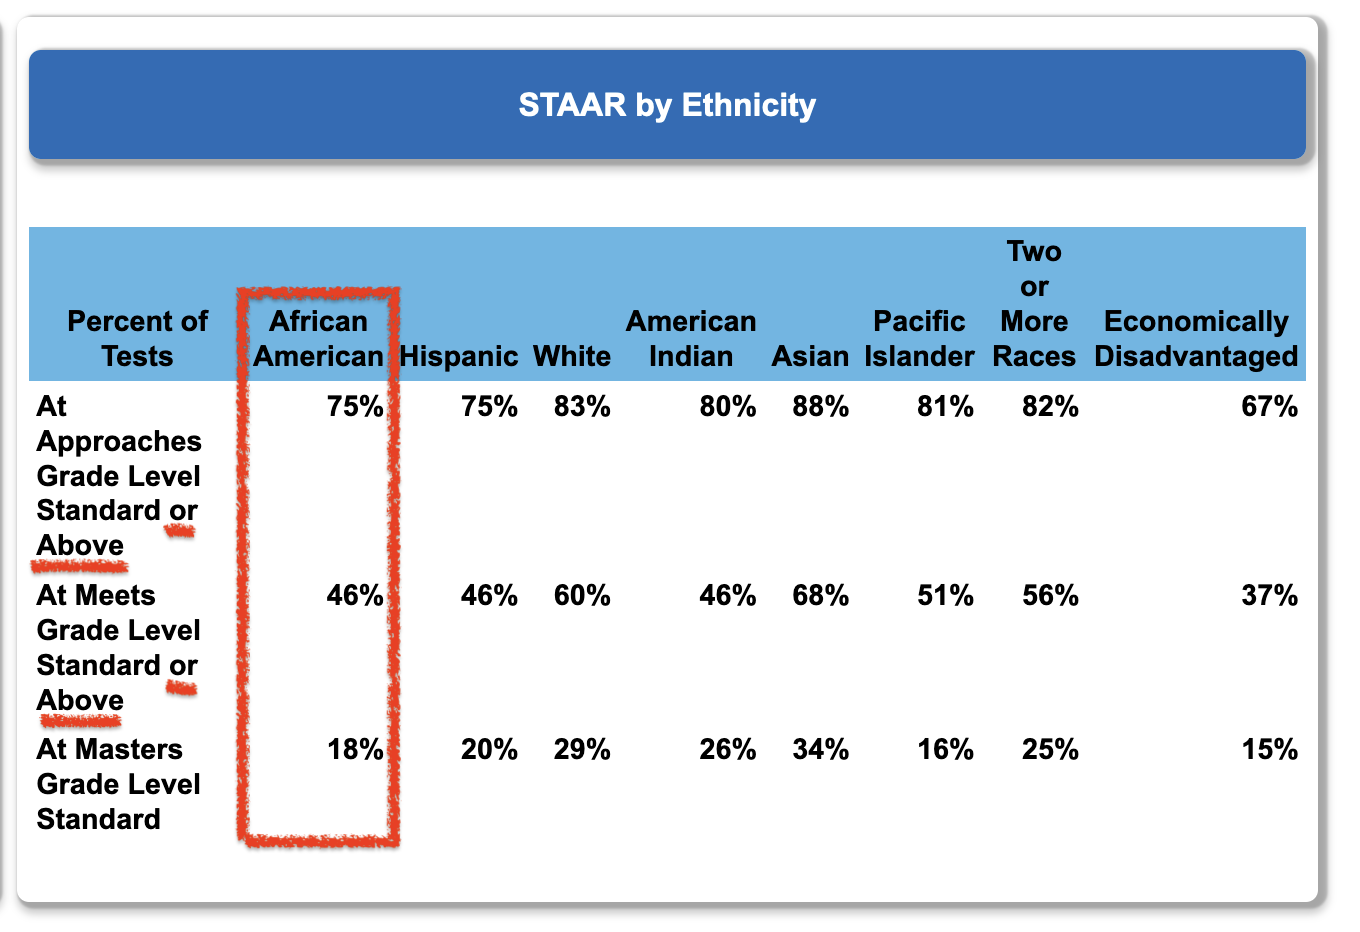
\includegraphics{img/staar-snapshot-by-ethnicity-2022-2023-annot.png}

Fig: The first two rows combine more than one achievement level

\vspace{0.3in}

\subsection{\texorpdfstring{\textbf{OBSTACLE
\#2}}{OBSTACLE \#2}}\label{obstacle-2}

These \textbf{\emph{`description-only'}} reports are `ill-suited' for
district improvement efforts for another reason: the TEA
`description-only' reports are \textbf{siloed by academic year}, making
it nearly impossible to create a time-period-by-time-period data frame
of any categories or levels the board may wish to analyze. In fact,
without time-period-by-time-period data \textbf{\emph{no meaningful
analysis is possible.}}

This siloing of academic years stands as a bristling obstruction to the
analysis of past performance and estimation of future results. Even the
least experienced board members intuitively know the importance of
numerical context when reviewing data for their district.

\begin{tcolorbox}[enhanced jigsaw, leftrule=.75mm, breakable, opacityback=0, toptitle=1mm, coltitle=black, opacitybacktitle=0.6, bottomrule=.15mm, colbacktitle=quarto-callout-note-color!10!white, colframe=quarto-callout-note-color-frame, arc=.35mm, bottomtitle=1mm, titlerule=0mm, title=\textcolor{quarto-callout-note-color}{\faInfo}\hspace{0.5em}{Note}, colback=white, rightrule=.15mm, left=2mm, toprule=.15mm]

It was our innate need for context that created the ``this-month vs
this-month-last-year vs year-to-date'' presentations so popular today.
``This vs that'' presentations are two-point comparisons that waste more
resources than all our unnecessary meetings put together.

\end{tcolorbox}

\vspace{0.3in}

\subsection{\texorpdfstring{\textbf{OBSTACLE
\#3}}{OBSTACLE \#3}}\label{obstacle-3}

\begin{tcolorbox}[enhanced jigsaw, leftrule=.75mm, breakable, bottomrule=.15mm, opacityback=0, colframe=quarto-callout-tip-color-frame, arc=.35mm, colback=white, rightrule=.15mm, left=2mm, toprule=.15mm]

``At sea one day you will smell land where there be no land.''

\bigskip

--- Elijah, to Ishmael and Queequeg

\emph{Moby Dick (film, 1956)}

\end{tcolorbox}

\vspace{0.3in}

Obstacle number 3 is not related to the TEA `description-only' reports
at all. It has to do with our human nature (or, as Jessica Rabbit put it
in the 1988 film `Who Framed Roger Rabbit': ``I'm not bad, I'm just
drawn this way!'').

For survival, humans evolved with the ability to rapidly detect
patterns. That instinct can lead us astray when studying our data.
Unfortunately, we quite naturally see `trends' and `signals' where there
are none.

Consider that for any three measurements there are at least 10
completely random arrangements that can arise. And, we have created
names to categorize these completely artificial `trends' that we think
we see:

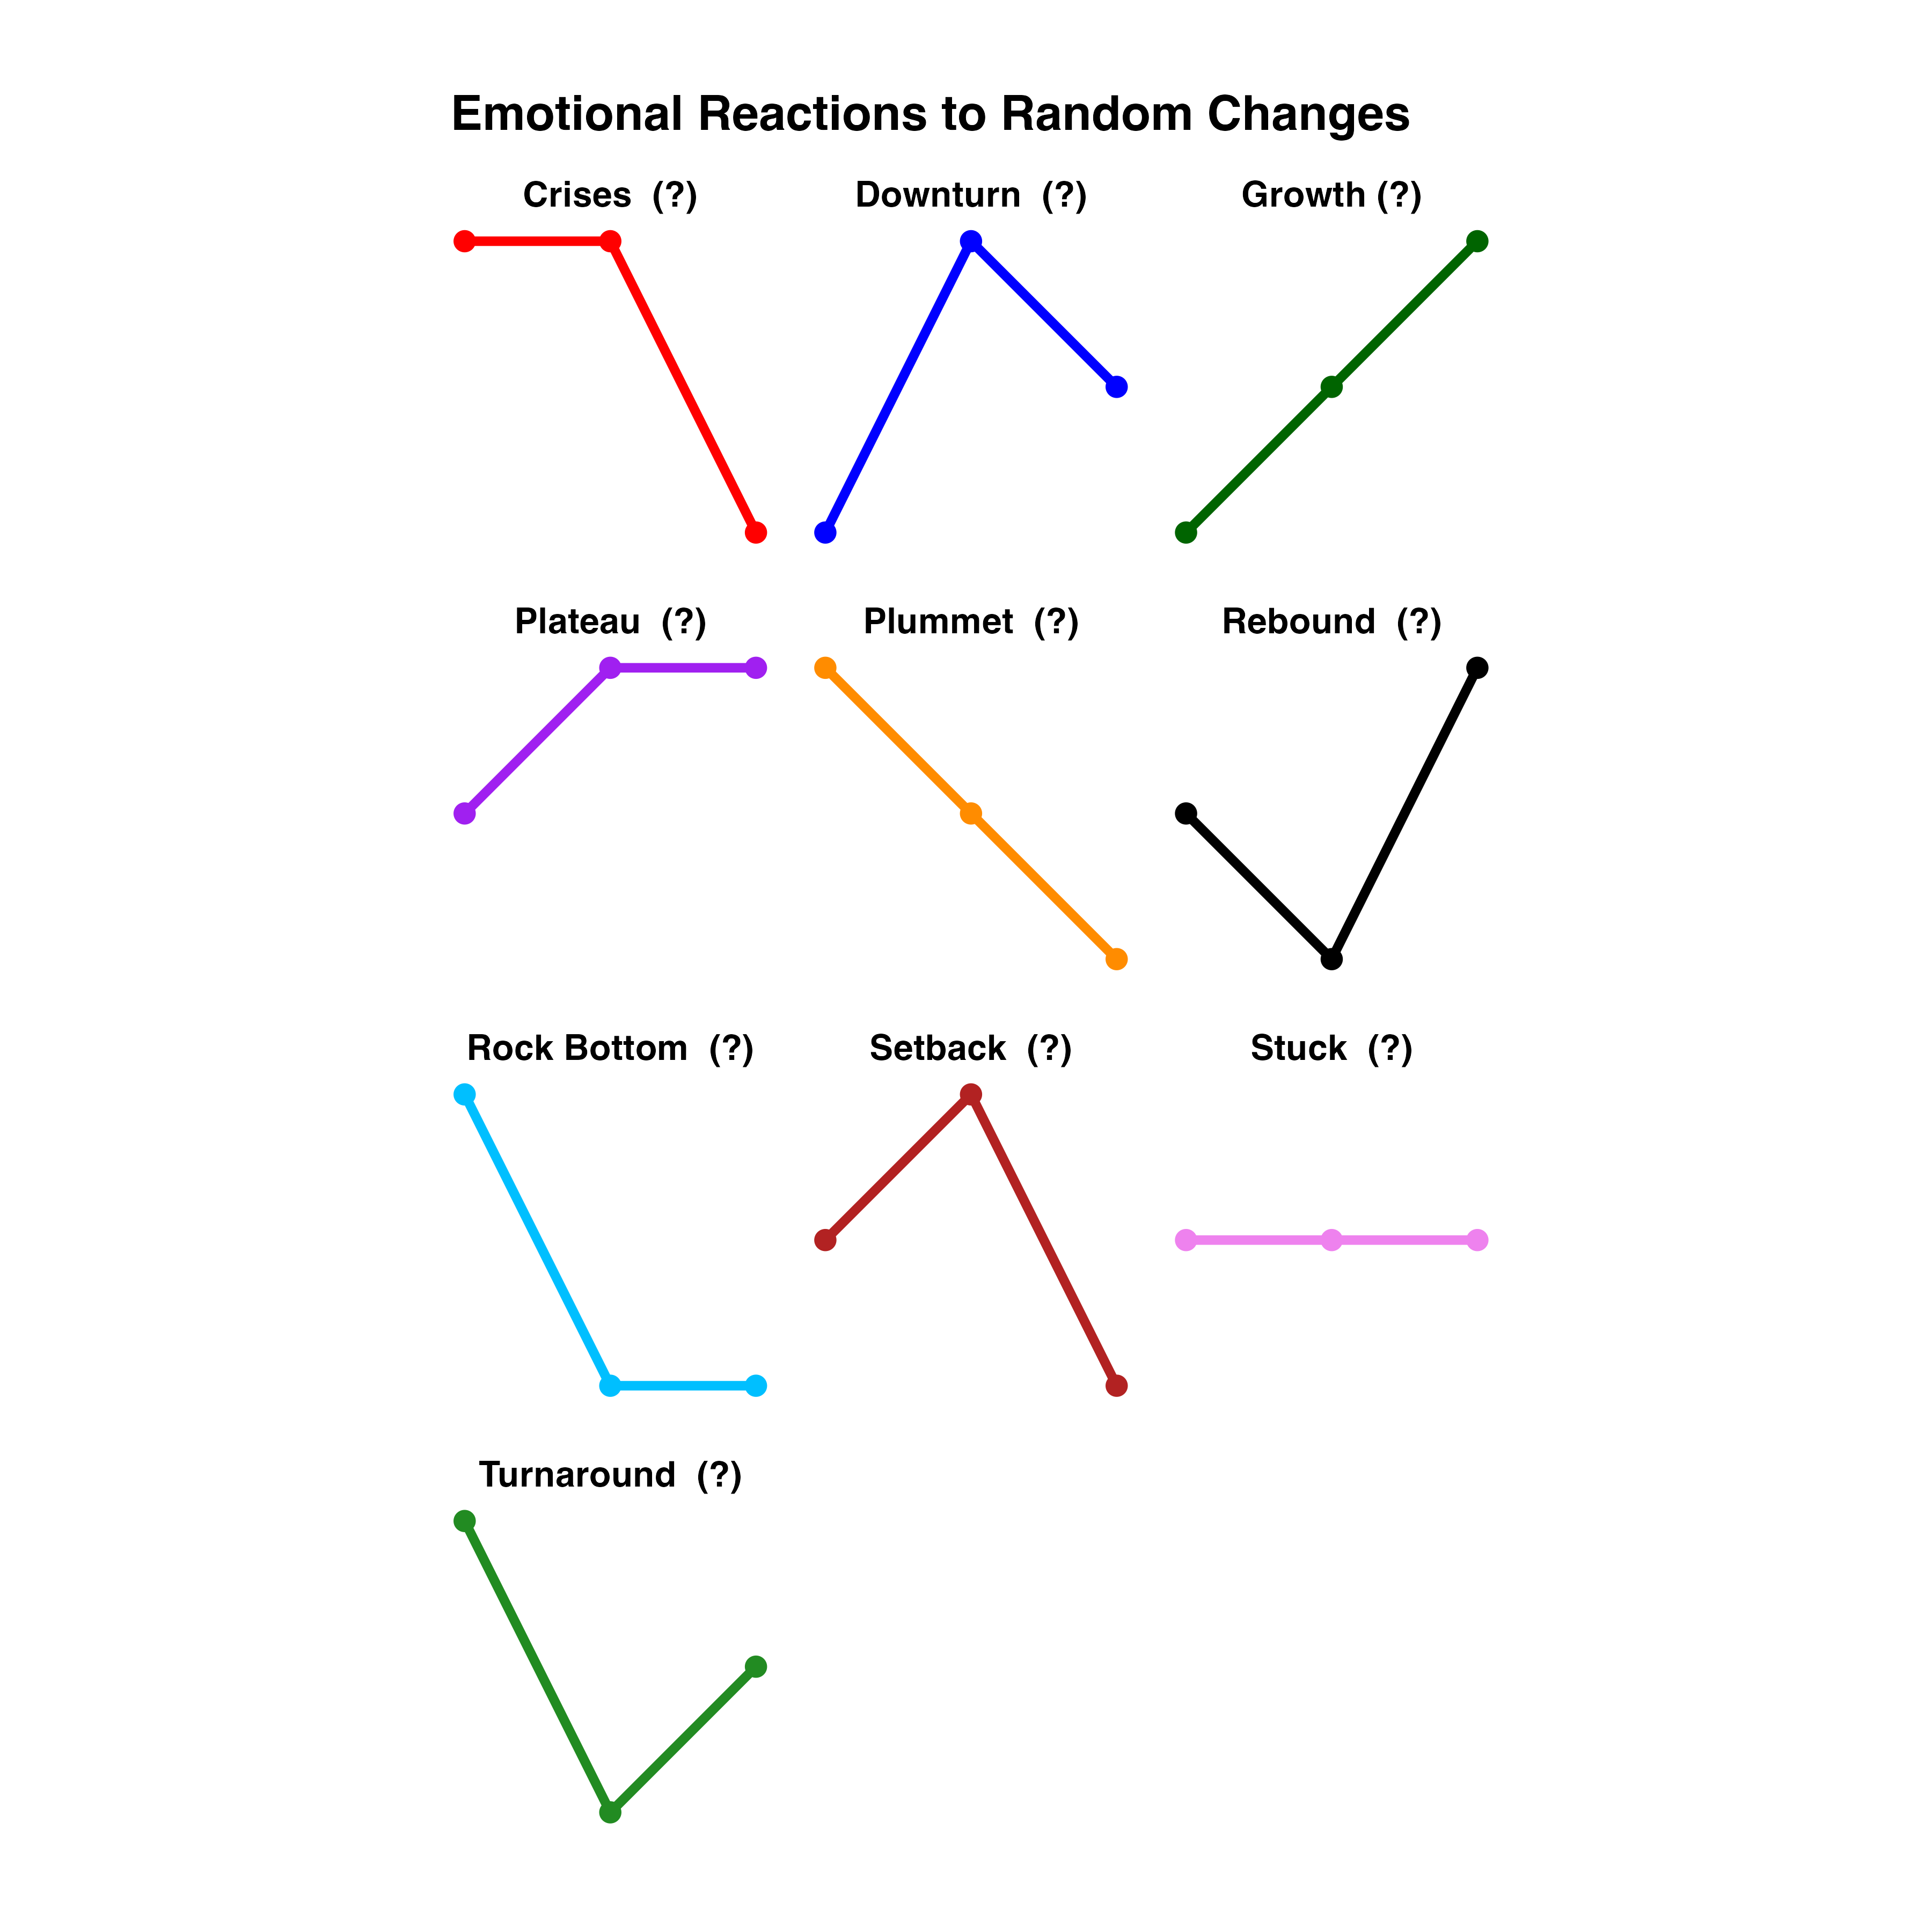
\includegraphics{img/10-random-arrangements-of-3-measurements.png}

Fig: Ten random arrangements of 3 measurements

\vspace{0.3in}

How many of those `trends' do you see in this example of TEA data placed
on a bar chart?

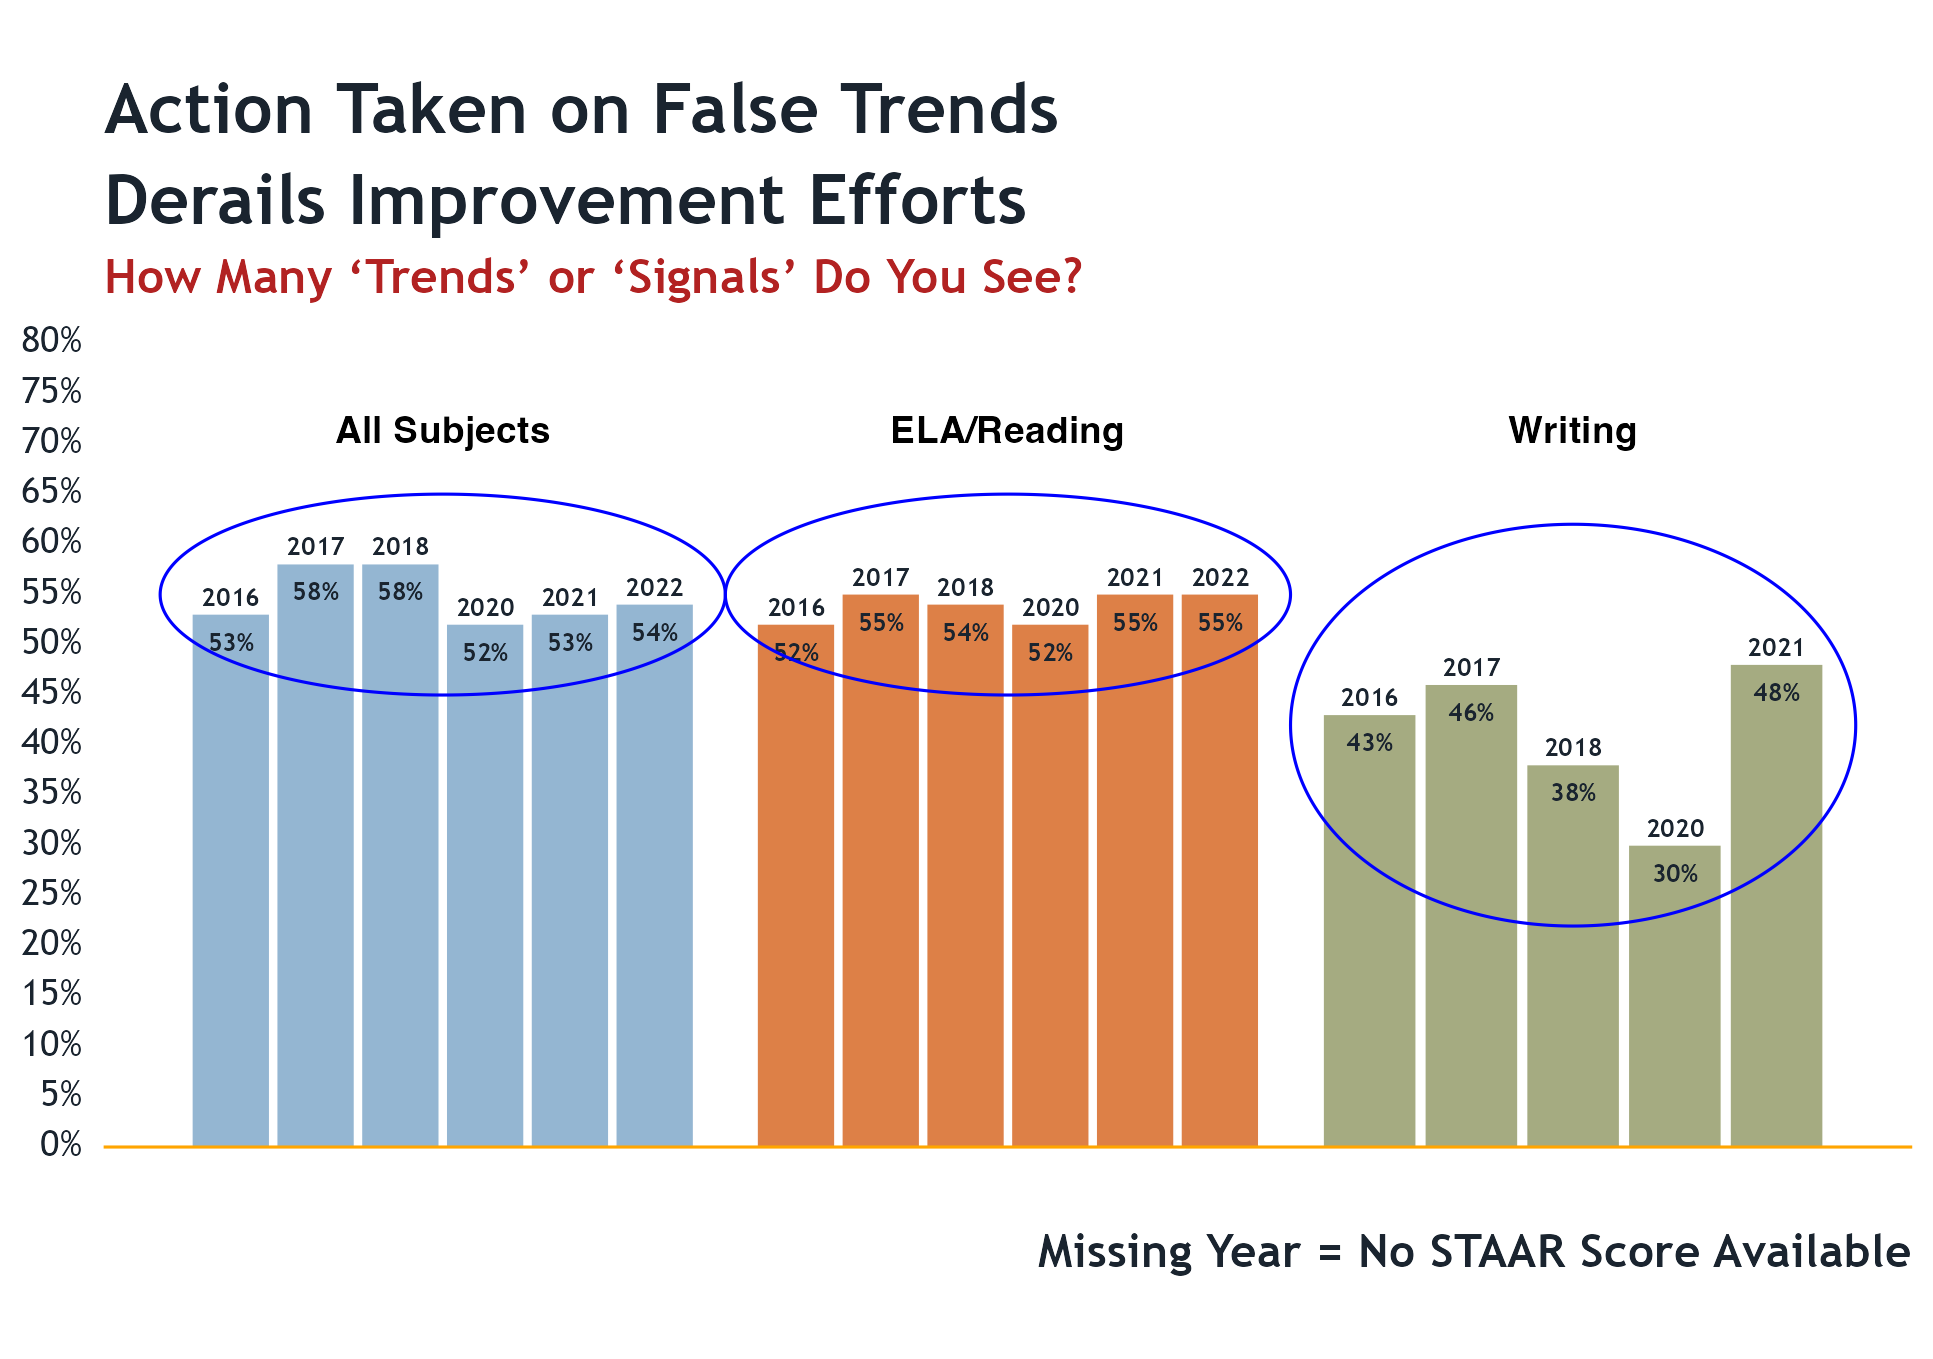
\includegraphics{img/false-signals-on-bar-charts.png}

Fig: Do you see any trends or signals in the bars?

\vspace{0.3in}

So, \textbf{\emph{we need a report that can separate the `common cause'
variation (routine variation) from the `special cause' variation that
signals a true trend, or a detectable event that changes the system.}}

Our current \textbf{\emph{`description-only'}} reports do not make that
separation for us.

\vspace{0.3in}

\textbf{\emph{The XmR chart does.}}

\vspace{0.3in}

\subsection{\texorpdfstring{\textbf{OBSTACLE
\#4}}{OBSTACLE \#4}}\label{obstacle-4}

Obstacle \#3 is about our perceptions. Obstacle \#4 is about our
emotions. We have a very human impulse to intervene any time we feel
something is `wrong' and needs to be `fixed.' The incentives for board
members to seek interventions are many and varied, but it is the type of
change proposed that really matters.

This is also a situation where board members must remain vigilant about
getting involved in matters that are administrative (the responsibility
of the superintendent) and not district policy (the responsibility of
the board).

A problem arises if we react to a result that is merely random
(`common-cause' variation) as if it were a `special cause' signal. This
is called `tampering' and is \textbf{\emph{guaranteed to make things
worse.}} The variation we observe will increase and our good results
will be diluted accordingly. At worst, we can de-stabilize a stable
system that people have worked hard to develop.

This can be particularly acute when there is an incident involving
misfortune or safety. Although rare, these events may be quite
distracting and upsetting. However, trying to keep unpleasant events
from `ever happening again' is impossible and can make things worse, not
better.

It is part of the leadership responsibility of boards to provide a
measured and rational response when misfortune comes our way. Knowing
about `common cause' and `special cause' variation can help us do that.

\vspace{0.3in}

\section{\texorpdfstring{\textbf{NEW INFORMATION TO HELP
US}}{NEW INFORMATION TO HELP US}}\label{new-information-to-help-us}

What makes these proposed new reports so powerful are three unique
features:

\begin{enumerate}
\def\labelenumi{\arabic{enumi}.}
\item
  Prior period results for the process are \textbf{\emph{plotted in time
  order}}, oldest to newest, left to right (the more time periods
  presented the better). This is called \textbf{\emph{context}} and
  permits comparing our inputs to the outputs (results).
\item
  An average (or median) for the entire group of results, plotted as a
  center line. If the process is stable, this is the \textbf{\emph{best
  estimate for future results.}}
\item
  One simple calculation that sets the upper and lower bounds of results
  we can reasonably expect in the future. This is called
  \textbf{\emph{analysis.}}
\end{enumerate}

\textbf{\emph{All we need are just those three things}}; context,
estimate of future performance, and analysis. All three use simple
arithmetic; not even algebra. But, none of the
\textbf{\emph{`'description-only'}} reports currently available have all
three elements. Usually, they have none of the three.

Accordingly, those \textbf{\emph{`description-only'}} reports cannot
answer the important questions. We are left with only a vague intuition
about what the data are trying to tell us. All too often intuition and
personal experience have proven to be unreliable guides for action on
policy, performance, and pedagogy.

\vspace{0.3in}

\section{\texorpdfstring{\textbf{ANALYSIS - WHAT IS
IT?}}{ANALYSIS - WHAT IS IT?}}\label{analysis---what-is-it}

Analysis was developed to help separate the actual signals in the data
from the random fluctuations that are always present in any measurement.

In this context analysis means to subject the data to \textbf{ONE} very
simple statistical test to see if the system (or process) producing the
data shows evidence of being in a \textbf{\emph{stable state}}, with a
\textbf{\emph{predictable output capability}}.

If stable, this output capability will show as a range of values that
constitute `normal' for the process. Until the process itself changes in
some fundamental way future measurements will wander between the
expected output limits; sometimes upward, sometimes downward, sometimes
the same.

\begin{tcolorbox}[enhanced jigsaw, leftrule=.75mm, breakable, opacityback=0, toptitle=1mm, coltitle=black, opacitybacktitle=0.6, bottomrule=.15mm, colbacktitle=quarto-callout-note-color!10!white, colframe=quarto-callout-note-color-frame, arc=.35mm, bottomtitle=1mm, titlerule=0mm, title=\textcolor{quarto-callout-note-color}{\faInfo}\hspace{0.5em}{Note}, colback=white, rightrule=.15mm, left=2mm, toprule=.15mm]

For those thinking about the additional work needed to provide an
anlysis like this when reporting data to the board, or to the public, or
to each other please note that once the data was wrangled
\textbf{\emph{it took less than 5 minutes to create the XmR chart}}
using a very inexpensive Excel add-in!

\end{tcolorbox}

\vspace{0.3in}

\section{\texorpdfstring{\textbf{OVERCOMING THE
OBSTACLES}}{OVERCOMING THE OBSTACLES}}\label{overcoming-the-obstacles}

As it turns out, creating the analytic reports we need is very simple -
\textbf{IF} we can get our data into the right form for analysis. By
reporting out results in the usual \textbf{\emph{`description-only'}}
formats, neither the Texas Education Agency (TEA) nor the Texas
Association of School Boards (TASB) appear to be able to help us with
this particular limitation. It is up to us to take control of our own
reporting needs.

\vspace{0.3in}

\section{\texorpdfstring{\textbf{GETTING BLOOD FROM THE
TURNIP}}{GETTING BLOOD FROM THE TURNIP}}\label{getting-blood-from-the-turnip}

After an embarrassing amount of time spent `data wrangling' I was able
to construct from the 5 available TEA `Snapshot'
\textbf{\emph{`description-only'}} reports, and 1 Texas Academic
Performance Report (TAPR) `description-only' report, a small
time-period-by-time-period data frame for STAAR scores for all
subject-matter categories at the district-level for the academic years
ended 2016-2022. (No STAAR scores were available for the 2019 academic
year.)

\vspace{1.0in}

The TEA STARR Data Divided Into Constituent Parts for the subject `Math'

\begin{longtable}[]{@{}cccccc@{}}
\caption{Subject = Math, with Proportions Broken Into Constituent
Parts.}\tabularnewline
\toprule\noalign{}
Year & Approaches & Mts Std & Masters & Combined & Failing \\
\midrule\noalign{}
\endfirsthead
\toprule\noalign{}
Year & Approaches & Mts Std & Masters & Combined & Failing \\
\midrule\noalign{}
\endhead
\bottomrule\noalign{}
\endlastfoot
2016 & 31\% & 29\% & 24\% & 84\% & 16\% \\
2017 & 27\% & 31\% & 30\% & 88\% & 12\% \\
2018 & 25\% & 29\% & 33\% & 87\% & 13\% \\
2020 & 29\% & 27\% & 23\% & 79\% & 21\% \\
2021 & 30\% & 27\% & 21\% & 78\% & 22\% \\
2022 & 31\% & 31\% & 18\% & 80\% & 20\% \\
\end{longtable}

An amazing amount of very useful information is now available to us
using just this small data frame.

\vspace{0.3in}

\section{\texorpdfstring{\textbf{FOOLED BY RANDOMNESS - AN EXTENDED
EXAMPLE}}{FOOLED BY RANDOMNESS - AN EXTENDED EXAMPLE}}\label{fooled-by-randomness---an-extended-example}

When looking at the results in the table above it would be difficult
\textbf{\emph{NOT}} to feel something about several categories,
particularly the changes observed in the `Masters Standard' and the
`Failing' columns. They seem large; and negative.

Like everyone else, I want some numerical context so I put the data in
the form of bar charts by year:

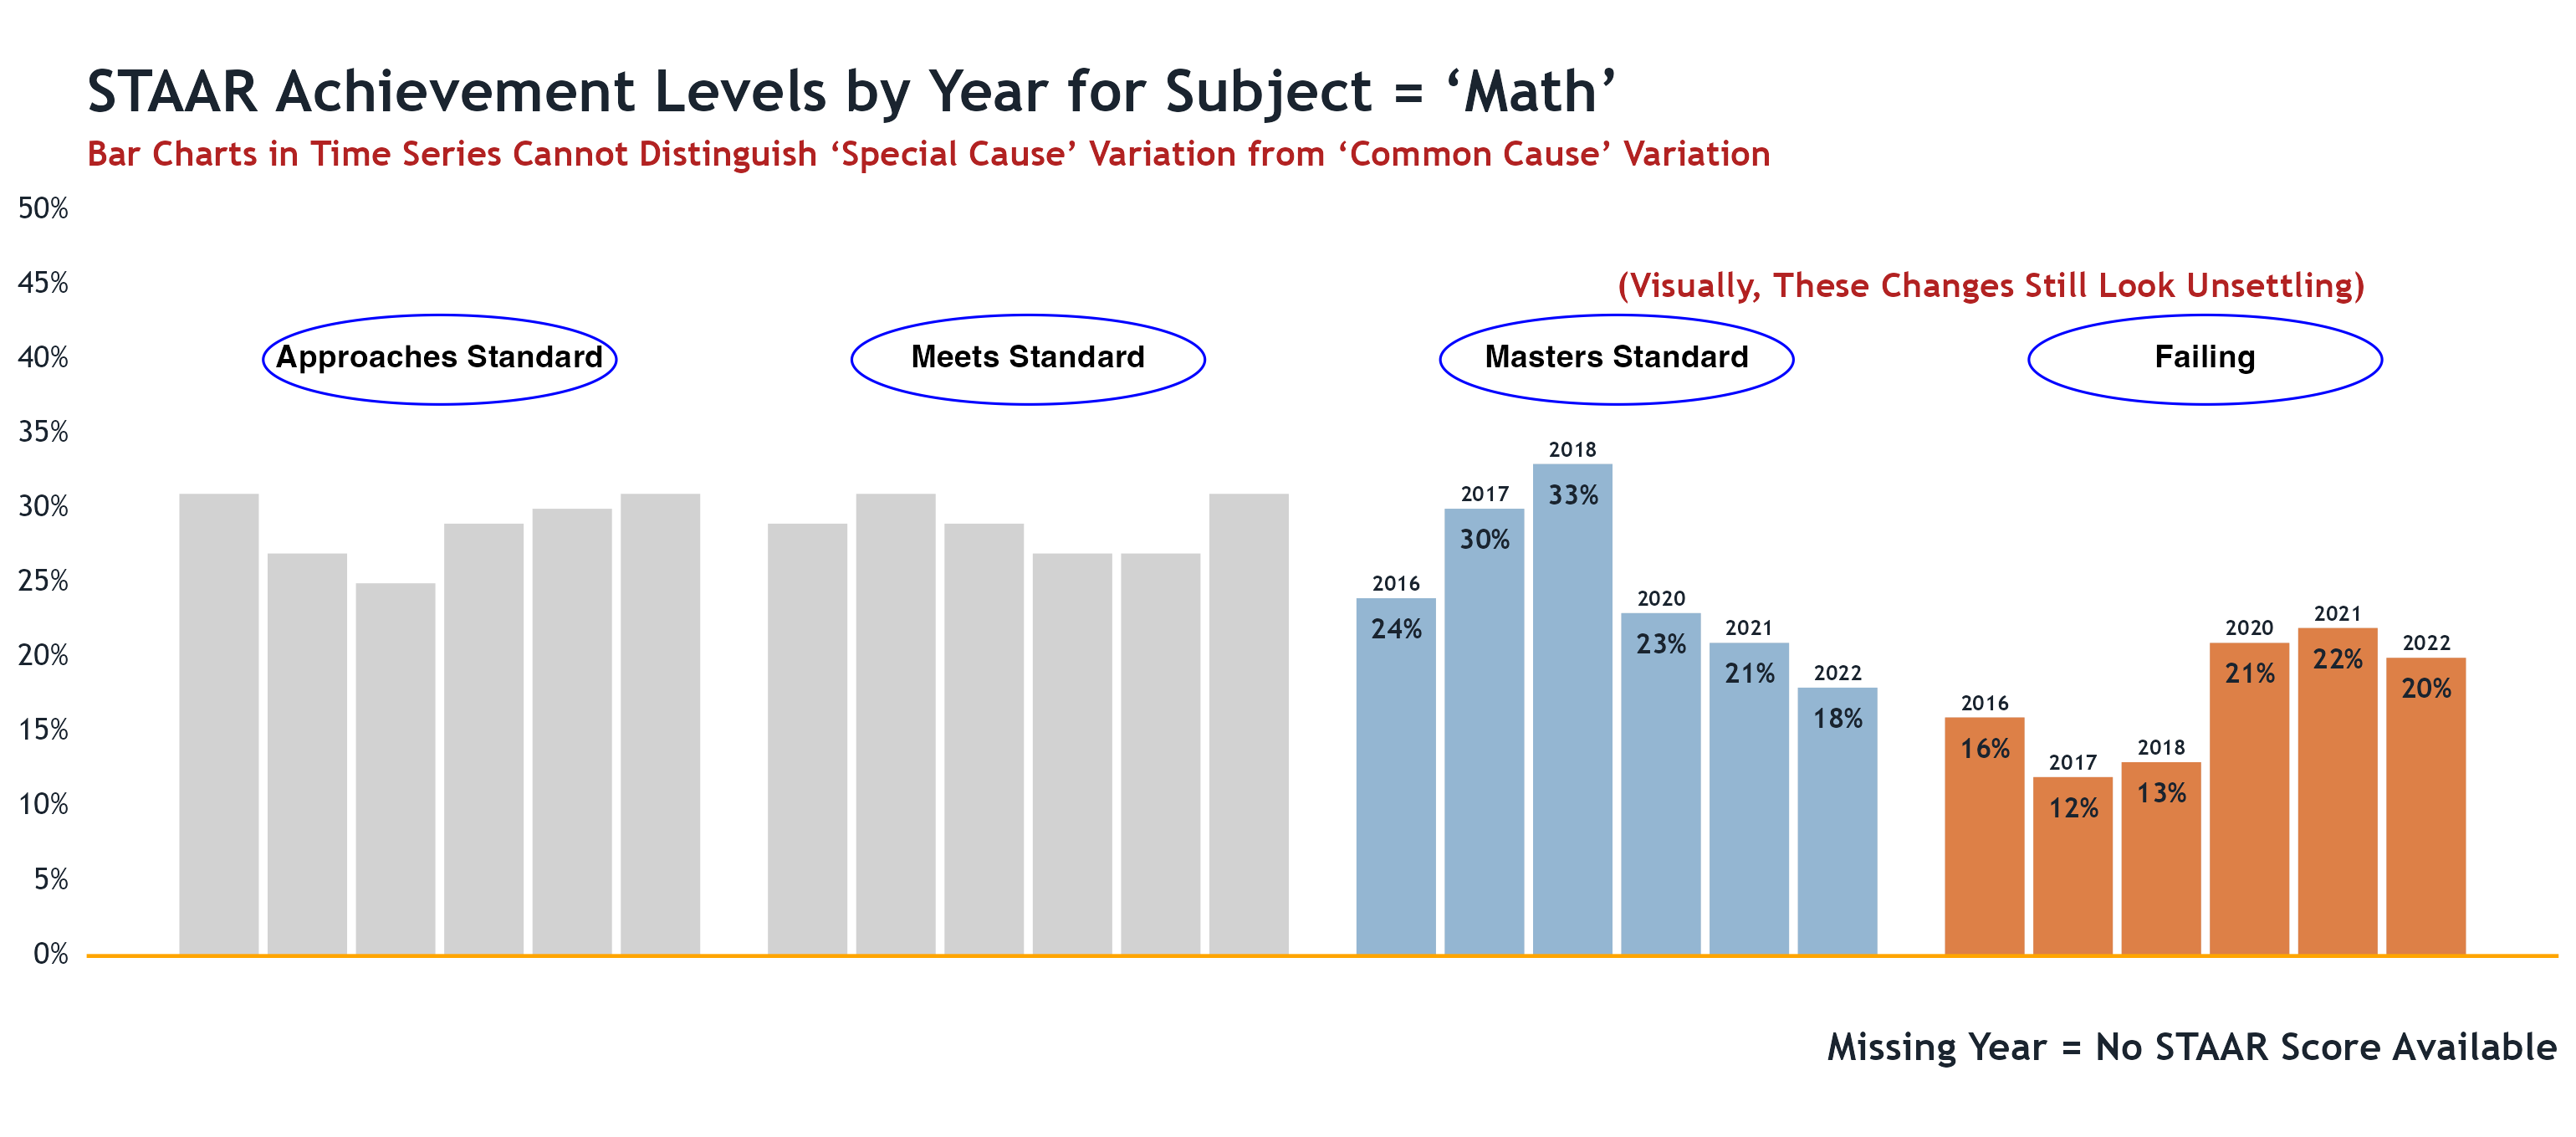
\includegraphics{img/staar-2016-2022-disagg-math-all-ratings-annot.png}

Fig: Data that is not grouped together taken from 5 TEA ``Snapshot''
description-only reports and 1 TAPR description-only report

\bigskip

\begin{tcolorbox}[enhanced jigsaw, leftrule=.75mm, breakable, opacityback=0, toptitle=1mm, coltitle=black, opacitybacktitle=0.6, bottomrule=.15mm, colbacktitle=quarto-callout-warning-color!10!white, colframe=quarto-callout-warning-color-frame, arc=.35mm, bottomtitle=1mm, titlerule=0mm, title=\textcolor{quarto-callout-warning-color}{\faExclamationTriangle}\hspace{0.5em}{Warning}, colback=white, rightrule=.15mm, left=2mm, toprule=.15mm]

I know from training and long experience that it is dangerous to rely
solely on visual inspection of data that is simply displayed and not
analyzed.

\end{tcolorbox}

\vspace{0.3in}

The XmR charts tell us a very different story.

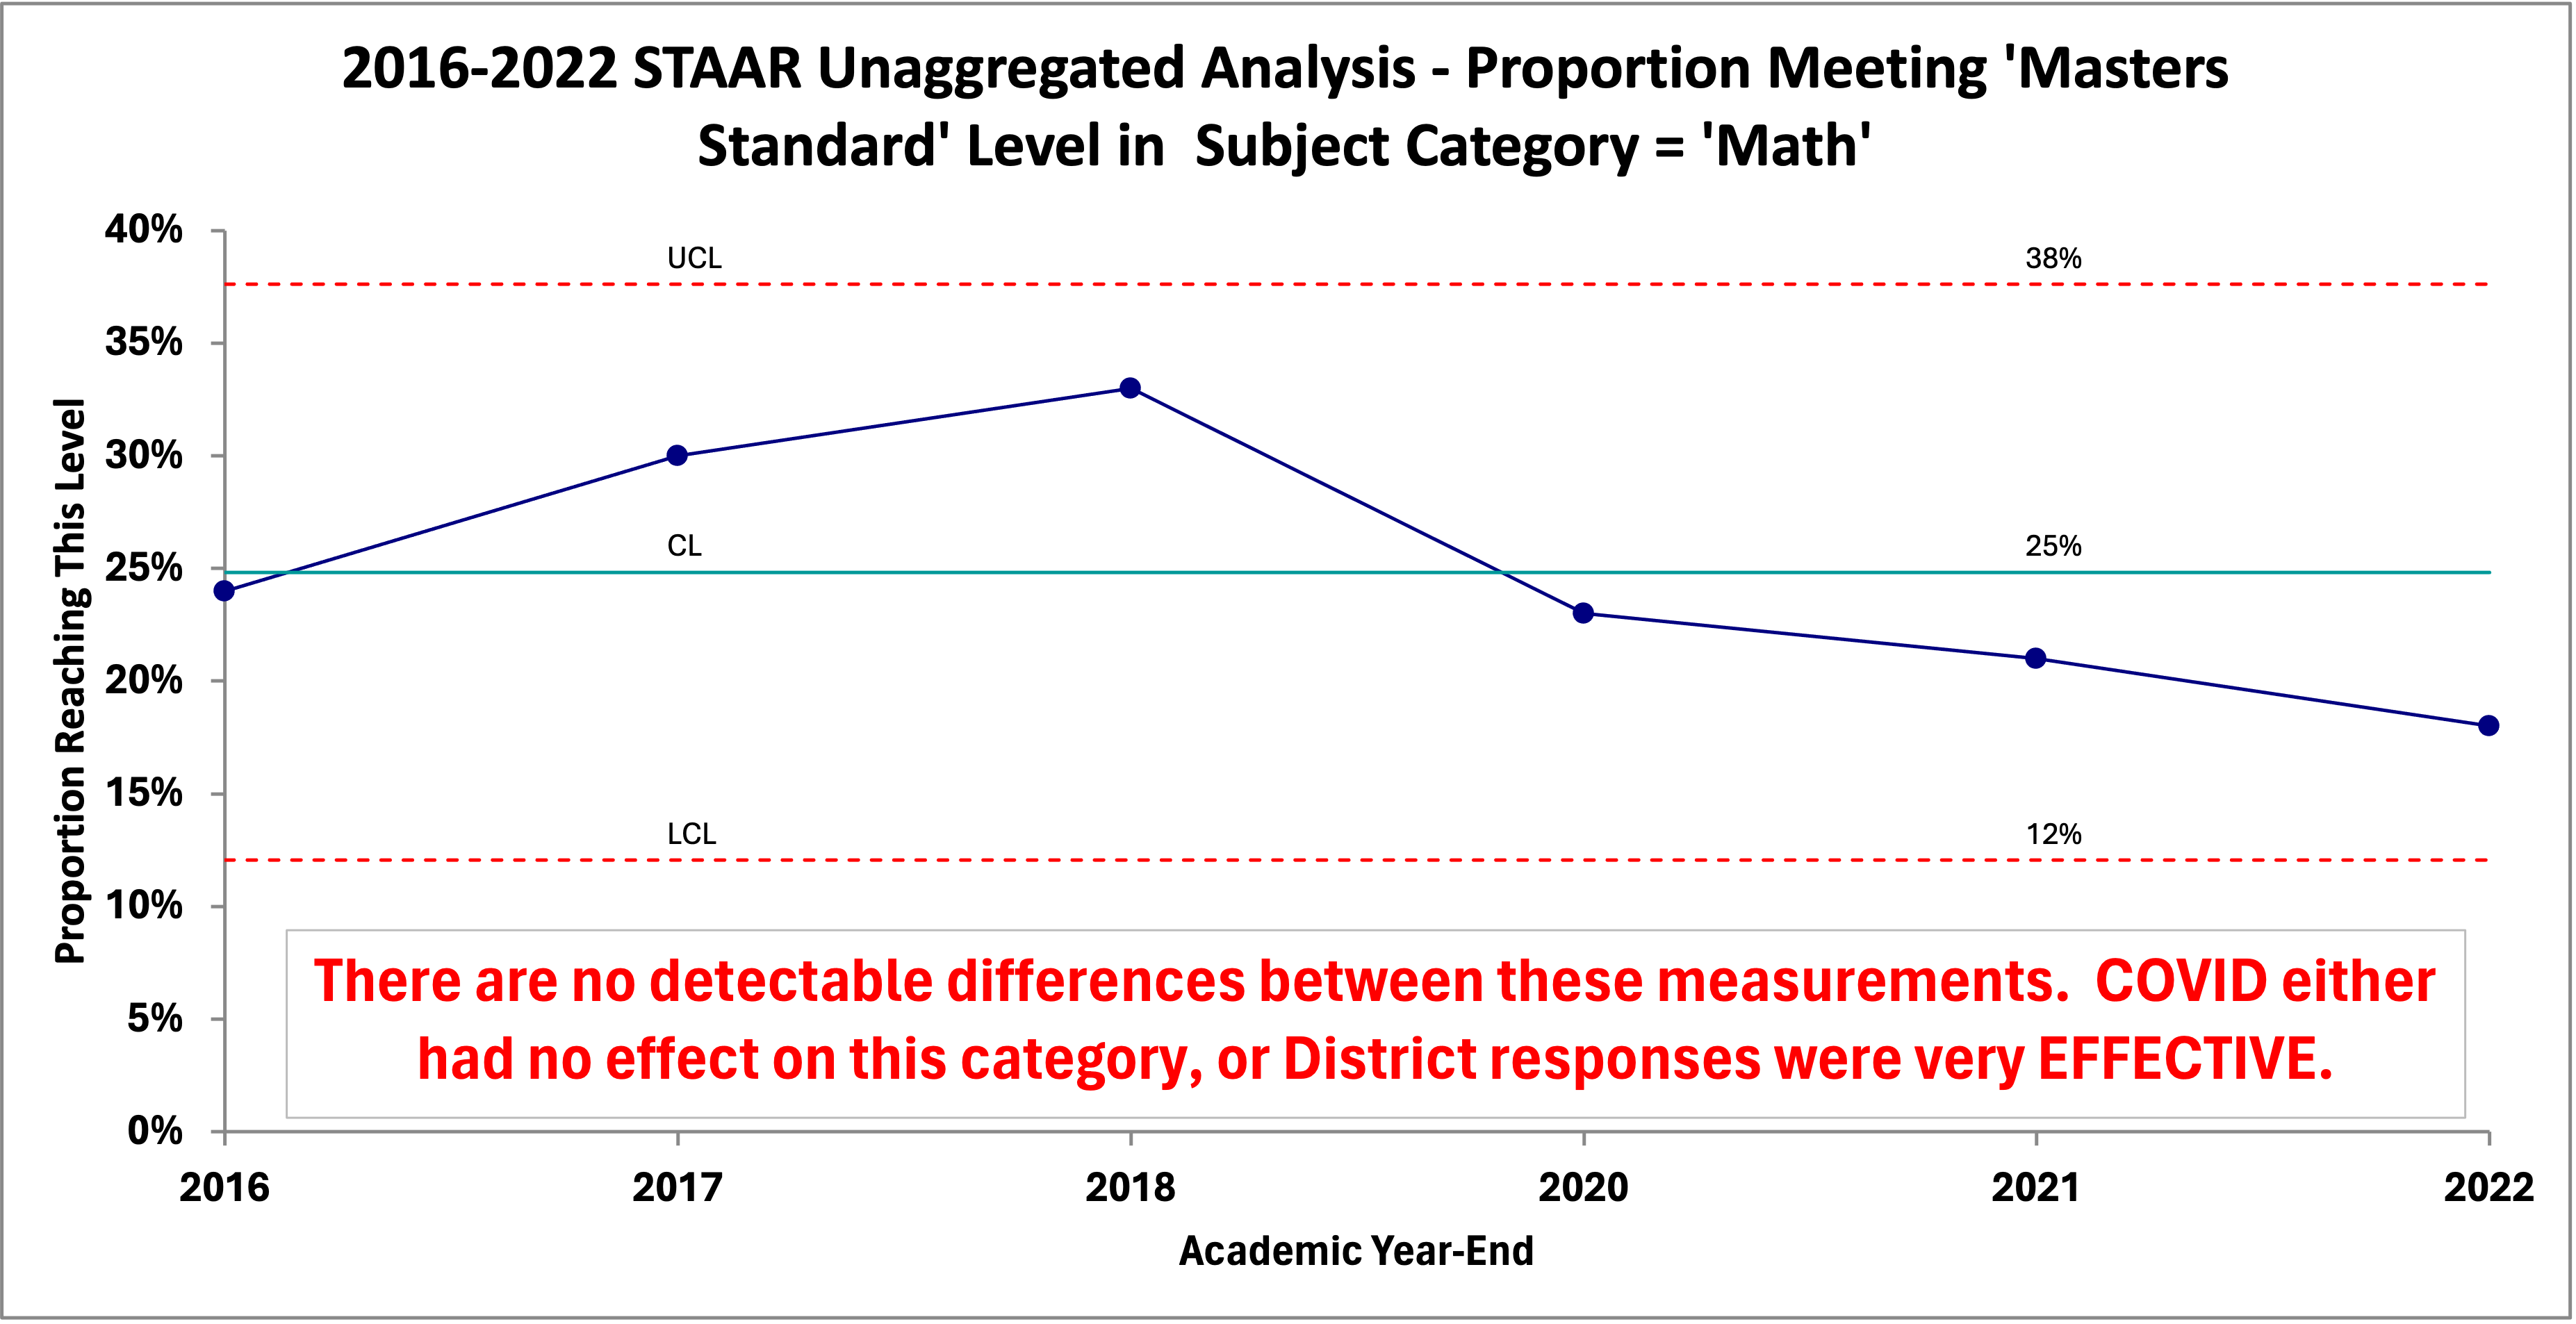
\includegraphics{pbc/xmr-2016-2022-math-masters-only.png}

Fig: Data taken from 5 TEA ``Snapshot'' description-only reports and 1
TAPR description-only report

\vspace{0.3in}

And, here's one TEA does not provide us that school boards would likely
be keenly interested in -- the `FAILING' column:

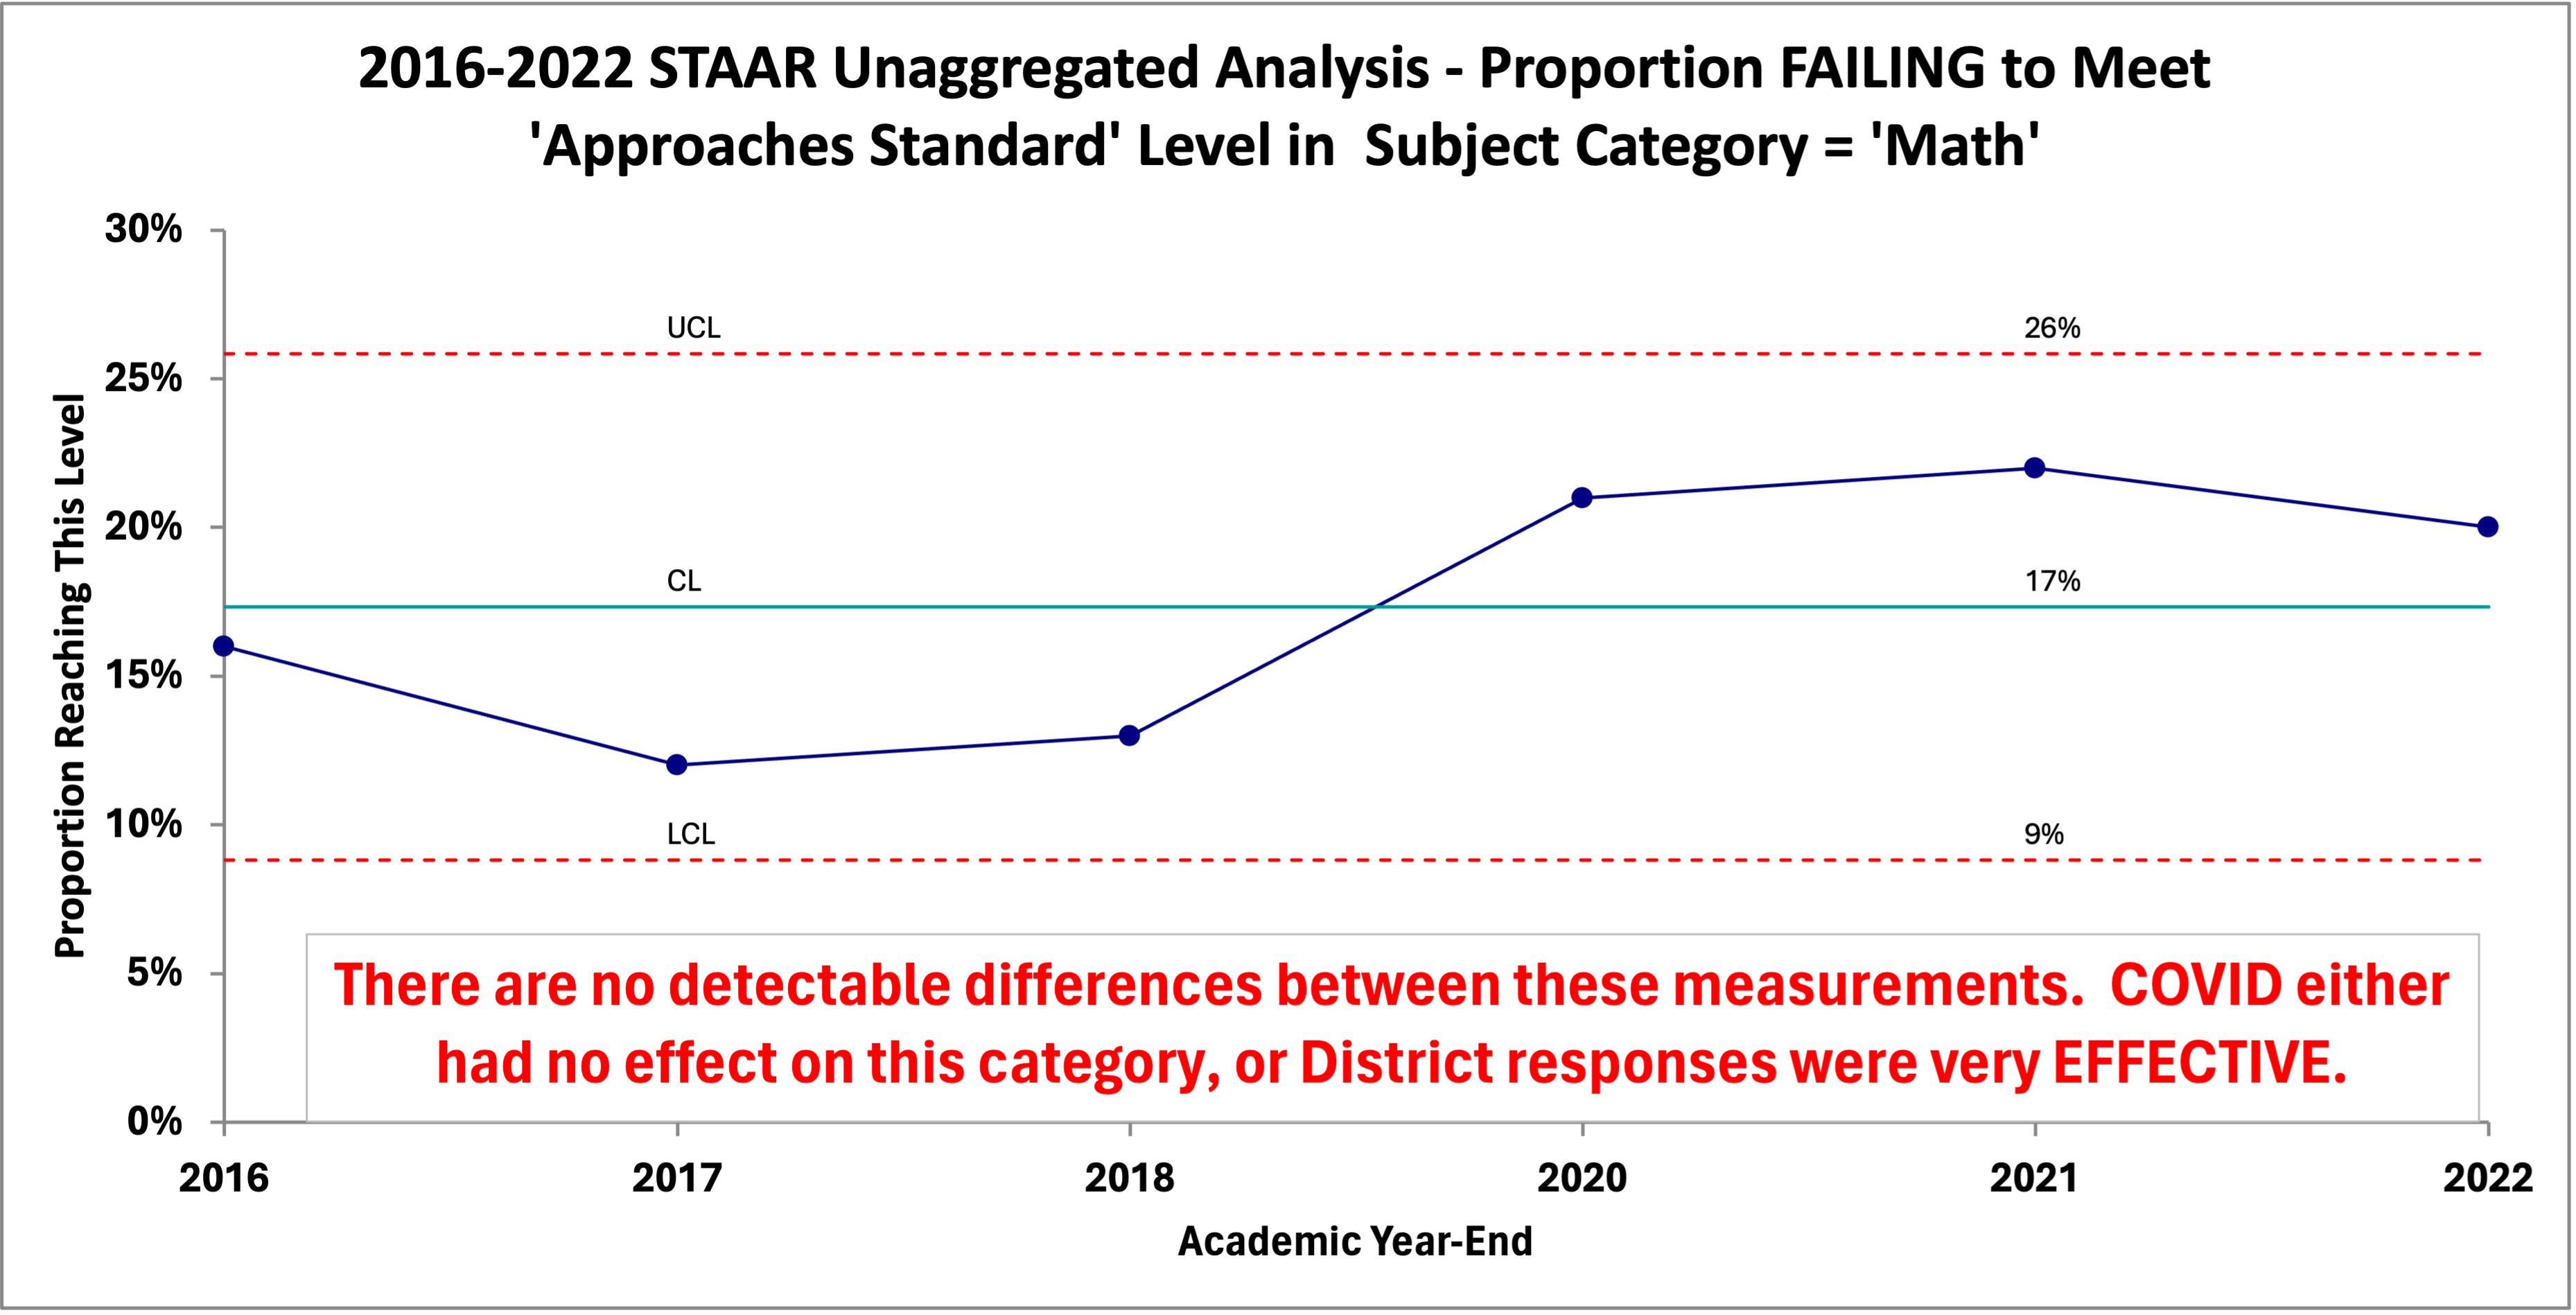
\includegraphics{pbc/xmr-2016-2022-math-failing.png}

Fig: Data taken from 5 TEA ``Snapshot'' description-only reports and 1
TAPR description-only report

\vspace{0.3in}

The following additional reports (XmR charts) use ungrouped data and
includes the necessary information to help us. Again, they cover public
STAAR data provided by TEA, along with a brief interpretation of the
charts taken as a whole. They provide a baseline (context) for
evaluating both past and future performance in these additional
categories and levels.

\vspace{0.3in}

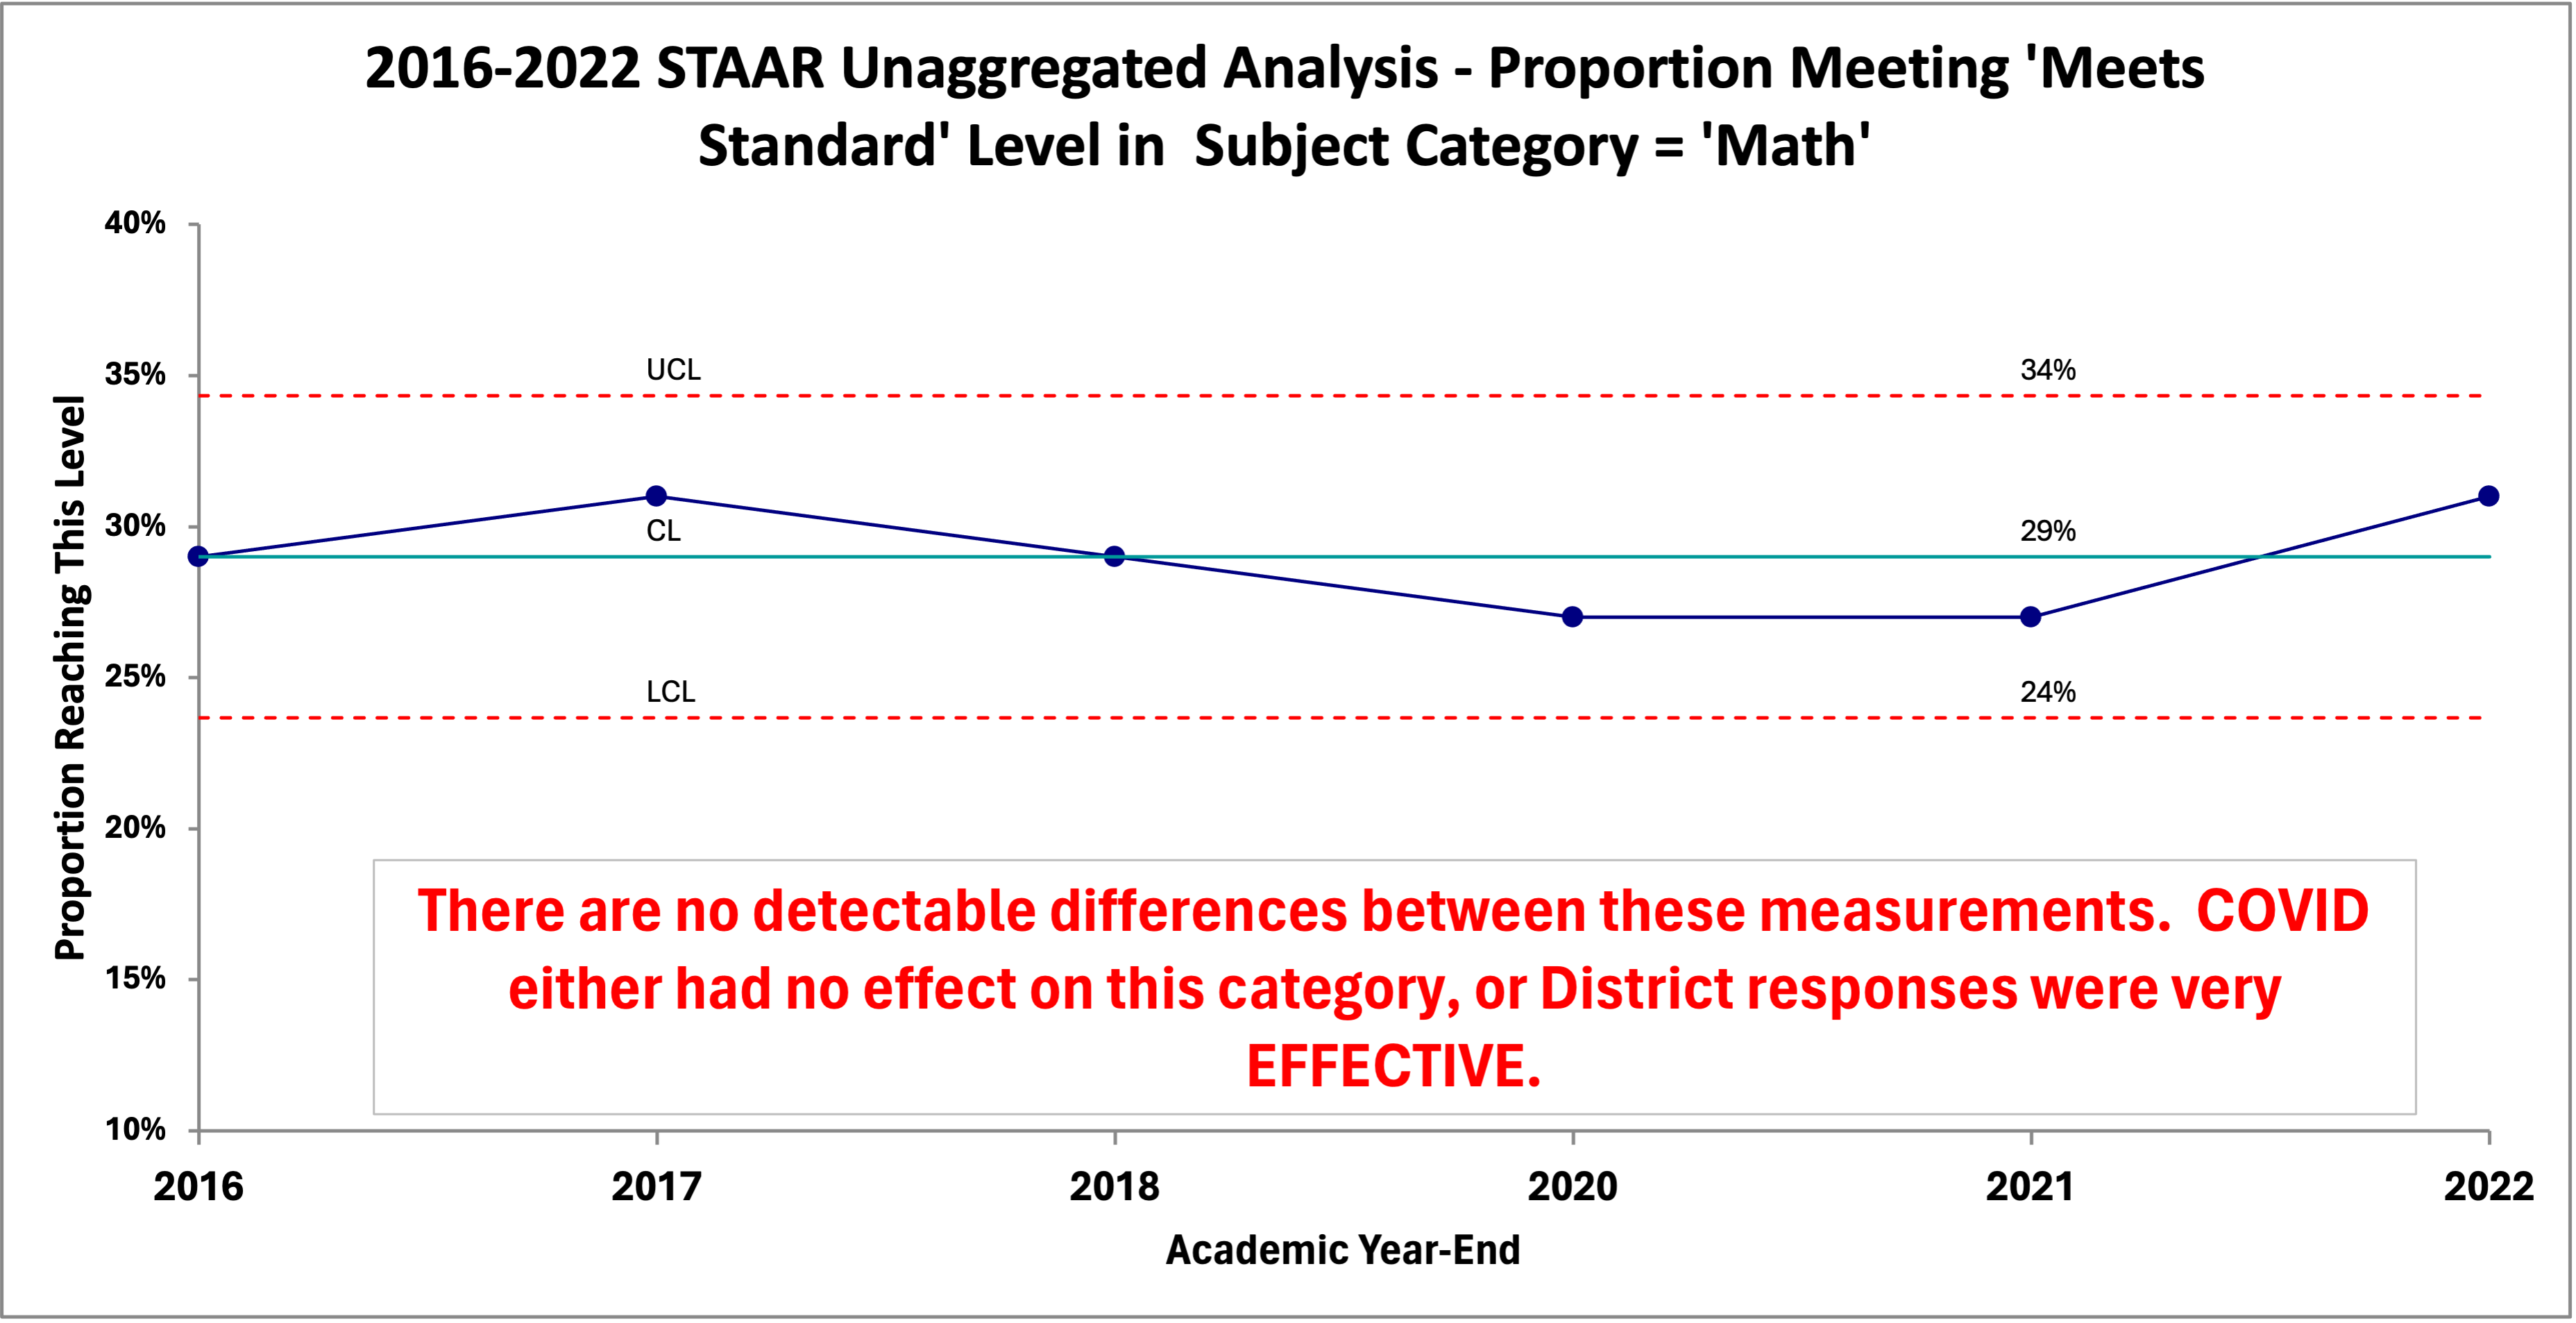
\includegraphics{pbc/xmr-2016-2022-math-meets-only.png}

Fig: Data taken from 5 TEA ``Snapshot'' description-only reports and 1
TAPR description-only report

\vspace{0.3in}

\subsection{INTERPRETING THE CHARTS}\label{interpreting-the-charts}

\begin{itemize}
\item
  The measurements do go up and down, but \textbf{\emph{there is no
  evidence that the movements are more than random variation}}. The ups
  and downs are almost certainly due to the many random forces acting on
  the cause system that produced the results. All display
  \textbf{\emph{common cause variation}} because the forces creating the
  ups and downs are common to all the results we see.
\item
  In this case, the charts show that all measurements fall between the
  calculated Upper Limit (UCL) and Lower Limit (LCL), with no
  statistical trends identified. Accordingly, the processes are
  \textbf{\emph{stable}}, with a \textbf{\emph{predictable output
  capability}}. Of the many forces influencing the results, no one of
  them is predominant. If one force (or a small combination) was
  predominate the chart would reveal it.
\item
  If the process remains fundamentally the same, \textbf{\emph{the
  proportion of students in the district taking the STAAR exam in Math
  that reach the level of `Meets Grade Level Standard, Masters Grade
  Level Standard, or Failed to Reach Approaches Grade Level Standard'
  will continue to fluctuate between their respective upper and lower
  control limits (UCL and LCL). Their averages are the best estimated of
  performance in the future.}}.
\item
  Any expectation of results outside those limits, without a significant
  change to the system, \textbf{\emph{would not be justified - at all}}.
\item
  Any future result, if it falls inside the calculated boundaries
  \textbf{\emph{does not signify an increase or decrease in the
  performance of the process.}} The routine `ups' or `downs' do not mean
  we are doing better, or worse.
\item
  Confidence in the interpretation will \textbf{increase} as you add
  more data to the chart. For example, it would be helpful to add years
  prior to 2016 to see if our interpretation of the data changed.
\item
  This charts includes all the information this data can reveal.
  \textbf{\emph{If you need or want more information you have to collect
  more data}}.
\end{itemize}

\begin{tcolorbox}[enhanced jigsaw, leftrule=.75mm, breakable, opacityback=0, toptitle=1mm, coltitle=black, opacitybacktitle=0.6, bottomrule=.15mm, colbacktitle=quarto-callout-tip-color!10!white, colframe=quarto-callout-tip-color-frame, arc=.35mm, bottomtitle=1mm, titlerule=0mm, title=\textcolor{quarto-callout-tip-color}{\faLightbulb}\hspace{0.5em}{\textbf{\emph{Technical Note For the Statistically Curious:}}}, colback=white, rightrule=.15mm, left=2mm, toprule=.15mm]

The calculated limits are NOT set at 3 standard deviations above and
below the average. The various statistical tests you learned in
Statistics 101 cannot help you when your attention is focused on the
future output of your district, campus, or pedagogy. They were designed
to characterize a population as it exists at a single moment in time -
how much or how many; without regard to why the population came to be
the way that it is. Even the forecasting techniques are inappropriate
for the task at hand.

\end{tcolorbox}

\vspace{0.3in}

\section{\texorpdfstring{\textbf{LEADERSHIP
REACTION}}{LEADERSHIP REACTION}}\label{leadership-reaction}

The content of your reports matter. The appropriate reaction of
management (which includes the school board) is \textbf{\emph{completely
different}} if the system or process indicates a \textbf{\emph{stable
state}} (predictable) than when it shows evidence of being in an
\textbf{\emph{unstable state}} (statistically speaking, of course).

Changing a stable process in reaction to so-called performance
indicators (KPIs) that fall within the `normal' range of a predictable
process is \textbf{\emph{harmful.}} It makes things
\textbf{\emph{worse}}; no matter how emotional you may become if you
think you see things `going in the wrong direction.'

Reacting to indicators falling outside the identified `normal' range is
\textbf{\emph{productive}}. If the indicator is in the `good' direction
efforts to identify the causes and duplicate them are almost always
successful. If they fall in the `bad' direction, efforts to identify the
causes and remove them are worthwhile.

\textbf{\emph{If your reports are `description-only' you cannot possibly
determine the most appropriate action for the circumstances.}}

\begin{tcolorbox}[enhanced jigsaw, leftrule=.75mm, breakable, opacityback=0, toptitle=1mm, coltitle=black, opacitybacktitle=0.6, bottomrule=.15mm, colbacktitle=quarto-callout-warning-color!10!white, colframe=quarto-callout-warning-color-frame, arc=.35mm, bottomtitle=1mm, titlerule=0mm, title=\textcolor{quarto-callout-warning-color}{\faExclamationTriangle}\hspace{0.5em}{\textbf{\emph{Cautionary Note:}}}, colback=white, rightrule=.15mm, left=2mm, toprule=.15mm]

Districts should cease dependence on recommendations for action based on
outside observational studies relying solely on correlations deemed
``statistically significant''. This so-called ``evidence based''
research is not based on generally accepted ``cause and effect''
experimental design. Despite the obligatory disclaimers, calls for
action often imply ``cause and effect'' relationships.\footnotemark{}

Remember, theories of a flat earth were ``evidence based'', as are most
stereotypes. The strength and quality of the evidence is more important
than whether there is any evidence at all. It is far better to see what
works in your district through the use of these methods and your own
efforts.

\end{tcolorbox}

\footnotetext{See for instance https://scholarworks.umt.edu/etd/1387/}

\vspace{0.3in}

Should we do nothing when we think we need a change?
\textbf{\emph{ABSOLUTELY NOT!}} However, \textbf{WHAT} we do and
\textbf{HOW} we do it is very different under each condition. Those who
simply want `change', without regard to whether or not the process is in
a stable state, will nearly always make things worse.

\vspace{0.3in}

\section{\texorpdfstring{\textbf{MAKE A DIFFERENCE, STARTING WHERE YOU
ARE}}{MAKE A DIFFERENCE, STARTING WHERE YOU ARE}}\label{make-a-difference-starting-where-you-are}

\begin{itemize}
\item
  We do not have to wait for TEA to begin providing data in the form we
  need it. We don't have to wait for TASB to offer training in the
  appropriate tools and methods to extract the new information we need
  for improvement.
\item
  It is ridiculously easy to plot dots in time order on a piece of paper
  and draw lines between the dots. Sally in fourth grade can do it. It
  takes very little training to learn how to construct and use an XmR
  chart.
\end{itemize}

\textbf{\emph{Here's a screenshot of a run chart made by 4th graders in
Leander ISD with newsprint and acrylic paint (and they can explain what
it means, too).}}

\vspace{0.3in}

\section{\texorpdfstring{\protect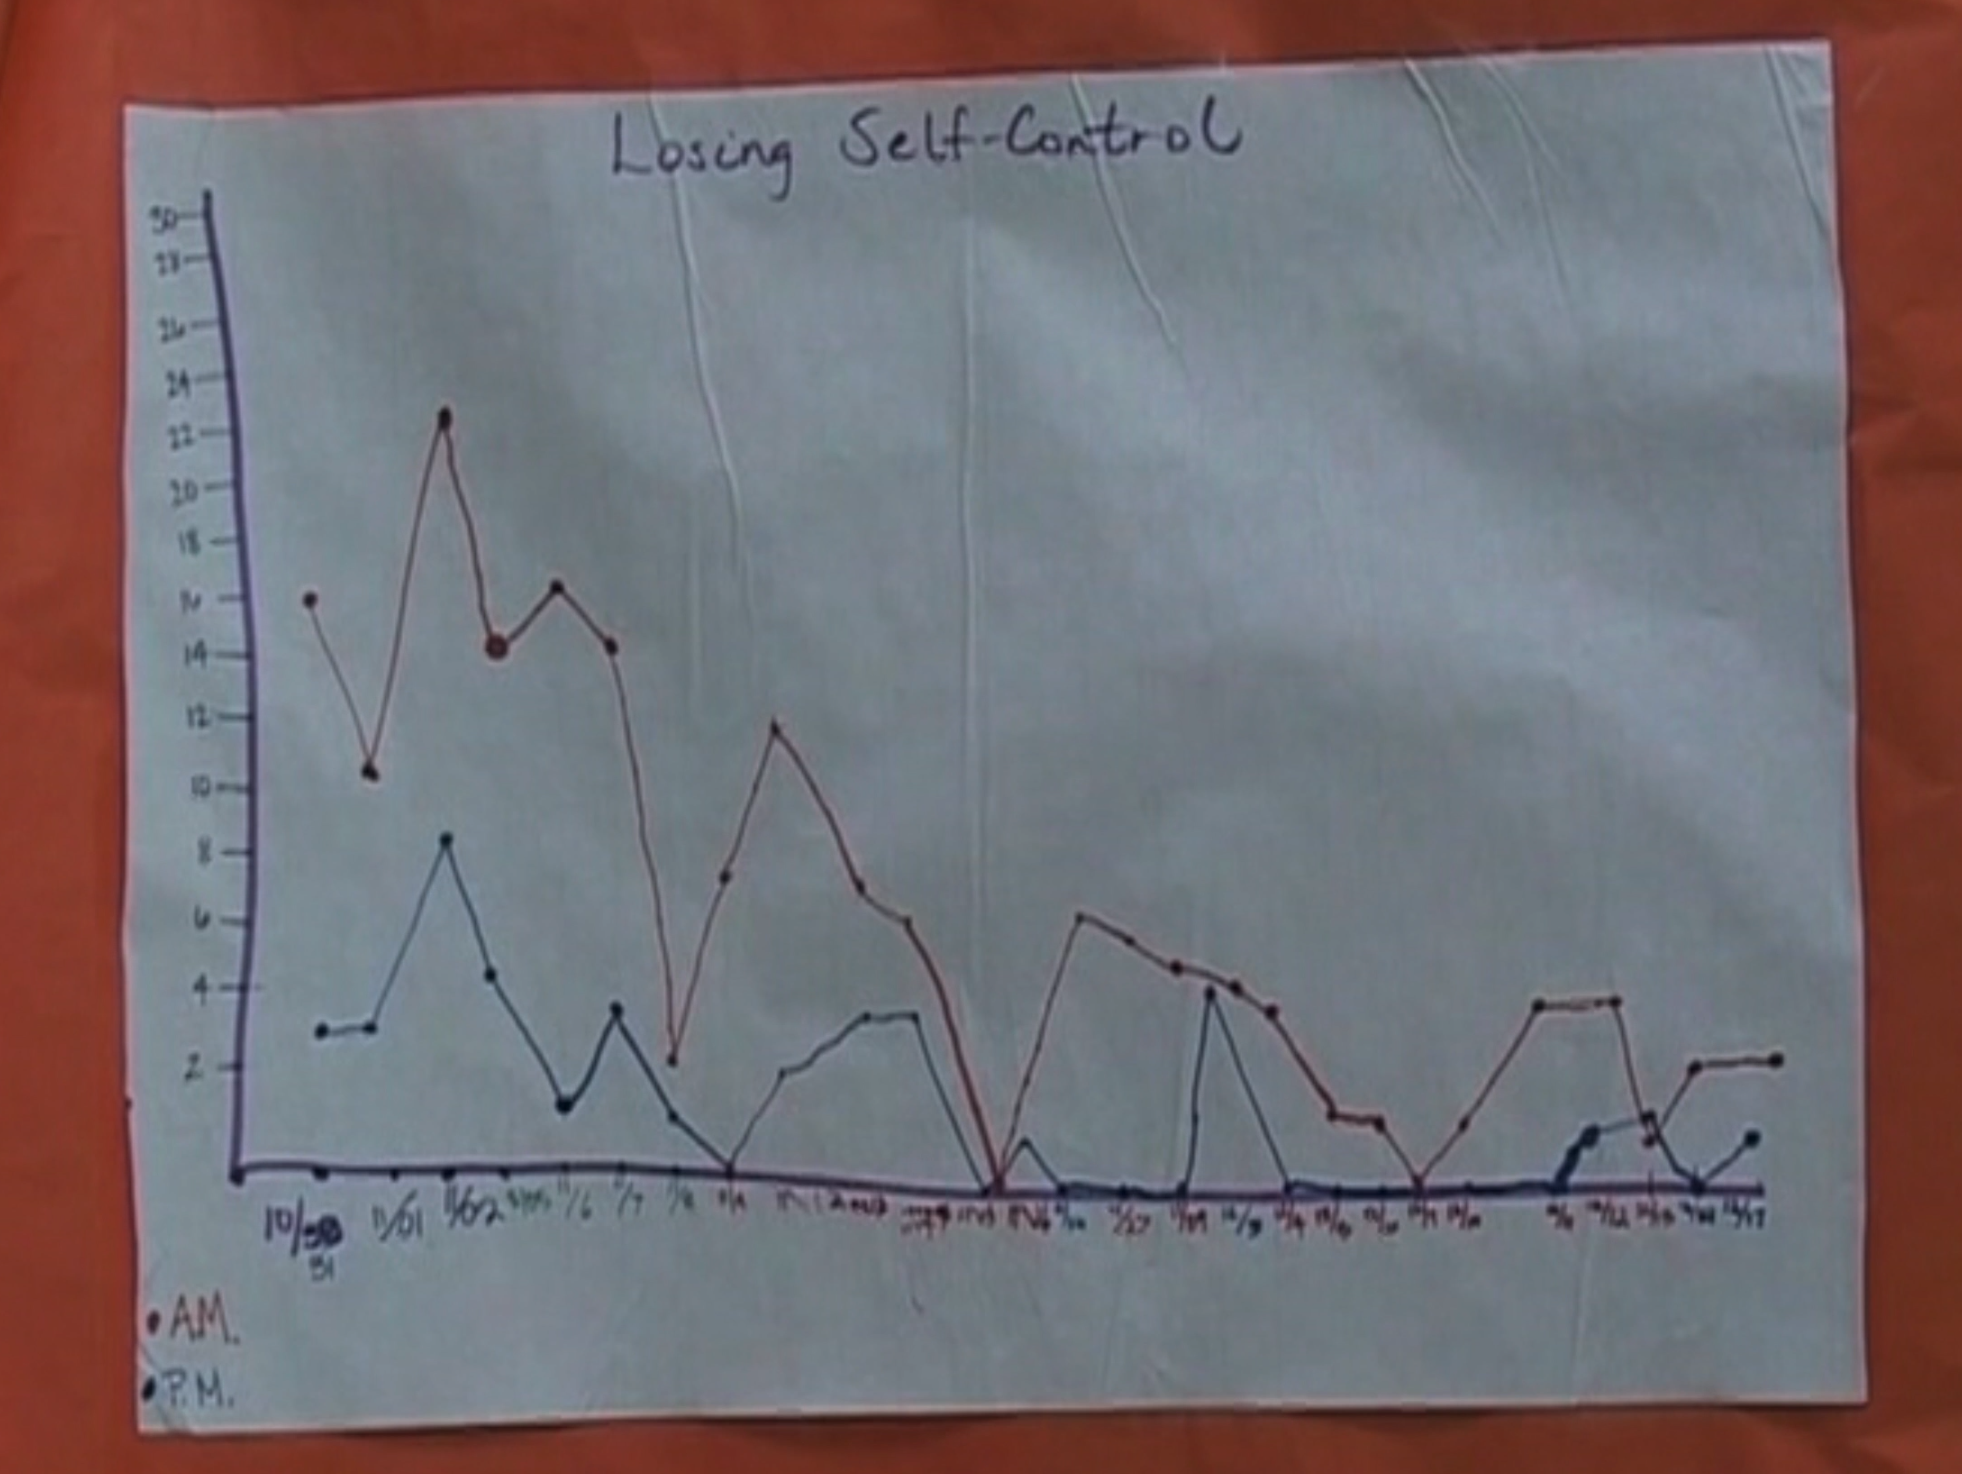
\includegraphics{img/leander-grade-4-run-chart.png}}{}}\label{section}

\vspace{0.3in}

When people in the organization begin `plotting the dots' amazing ideas
and insights bubble up from the people closest to the action - where it
is most valuable.

\begin{itemize}
\item
  You don't need to wait years to gather high-quality `baseline' data.
  In the real world data is never pristine. Use what you have now and
  improve future data collection as you go. You should strive to get as
  much data as possible but a valid analysis can be done with as few as
  6 data points (the ideal is 25 points, or more).
\item
  You don't have to have `everybody on board' to begin. Every district,
  department, function, and classroom generates data every day that can
  be used to help answer the big, important questions. Those interested
  in such questions can start now. Here are some examples:
\end{itemize}

\vspace{0.3in}

\subsection{\texorpdfstring{\textbf{SCHOOL
BOARDS}}{SCHOOL BOARDS}}\label{school-boards}

Metrics and goals defined in strategic plans, district improvement
plans, TEA scoring targets, safety and other district-level initiatives
can and should be assessed and evaluated with the aid of the new
information provided by an XmR chart. Even financial information can be
analyzed this way.

\vspace{0.3in}

\subsection{\texorpdfstring{\textbf{SUPERINTENDENTS \&
ADMINISTRATORS}}{SUPERINTENDENTS \& ADMINISTRATORS}}\label{superintendents-administrators}

Legacy programs and efforts to introduce new programs aimed at
improvement are all perfect candidates for this simple new chart.
Insight into campus-level issues (good and bad) are best analyzed with
the new information. Insight gathered this way helps answer questions
like, ``Is this initiative or program producing the results we want?''

\vspace{0.3in}

\subsection{\texorpdfstring{\textbf{CLASSROOMS}}{CLASSROOMS}}\label{classrooms}

Classroom attendance, MAP scores, disciplinary events, new pedagogues,
can be assessed with the aid of the new information. Anything a teacher
may be concerned about can quickly and easily be tracked and analyzed.

\vspace{0.3in}

\subsection{\texorpdfstring{\textbf{FUNCTIONAL
AREAS}}{FUNCTIONAL AREAS}}\label{functional-areas}

Facilities managers, bus drivers, custodians can ask and answer
questions such as:

\begin{itemize}
\item
  Are our initiatives to reduce utility costs working? By how much? At
  which campuses?
\item
  Are late-arrivals decreasing? Are disciplinary actions during travel
  increasing?
\item
  Can we reduce supply costs without compromising quality? How
  frequently should restrooms be re-stocked? At which campuses?
\end{itemize}

\vspace{0.3in}

\section{\texorpdfstring{\textbf{SUMMARY}}{SUMMARY}}\label{summary}

To go from monitoring a system to improving a system we must move from a
`snapshot' point of view to an `analysis' point of view.
\textbf{\emph{They are two different jobs and require different theory,
tools and methods.}} That means the data we use for improvement must
include the context of time order, an estimate of future performance,
and a range of values we can think of as `normal' variation.

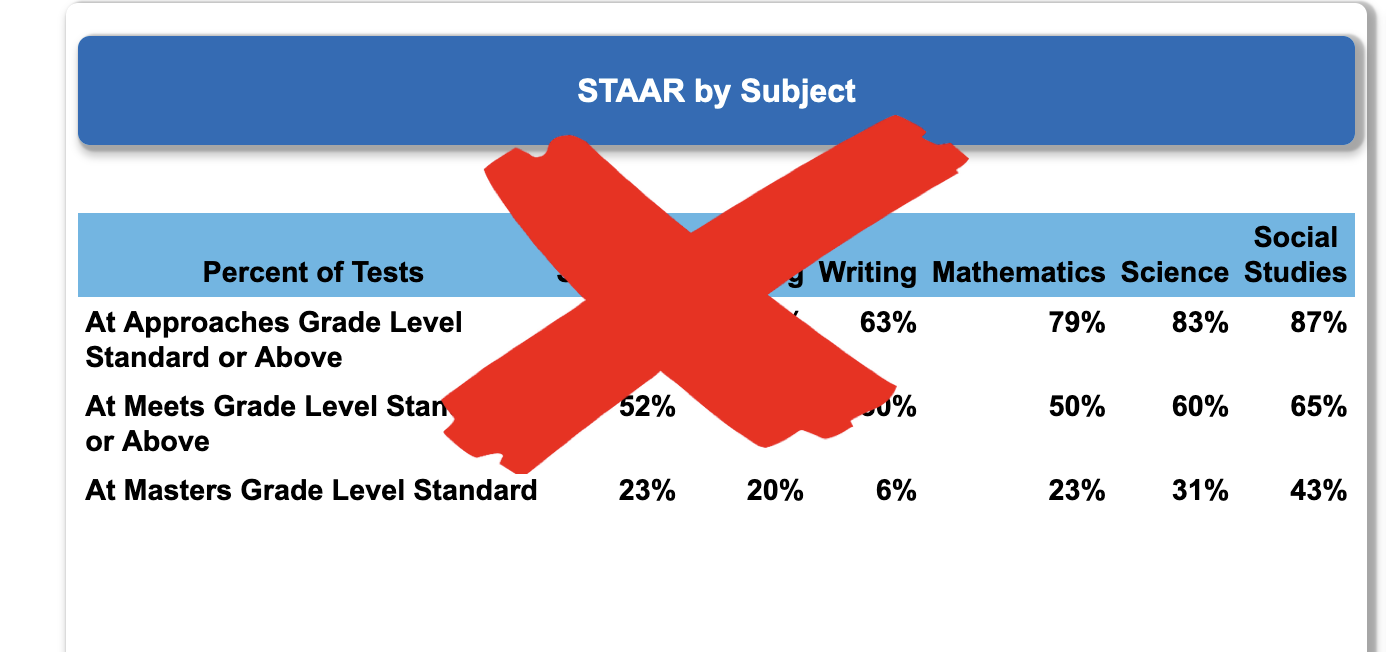
\includegraphics{img/crossed-out-staar-snapshot-by-subj-2022-2023-650-380.png}

Fig: This ``description-only'' form of report cannot help us to improve

\vspace{0.3in}

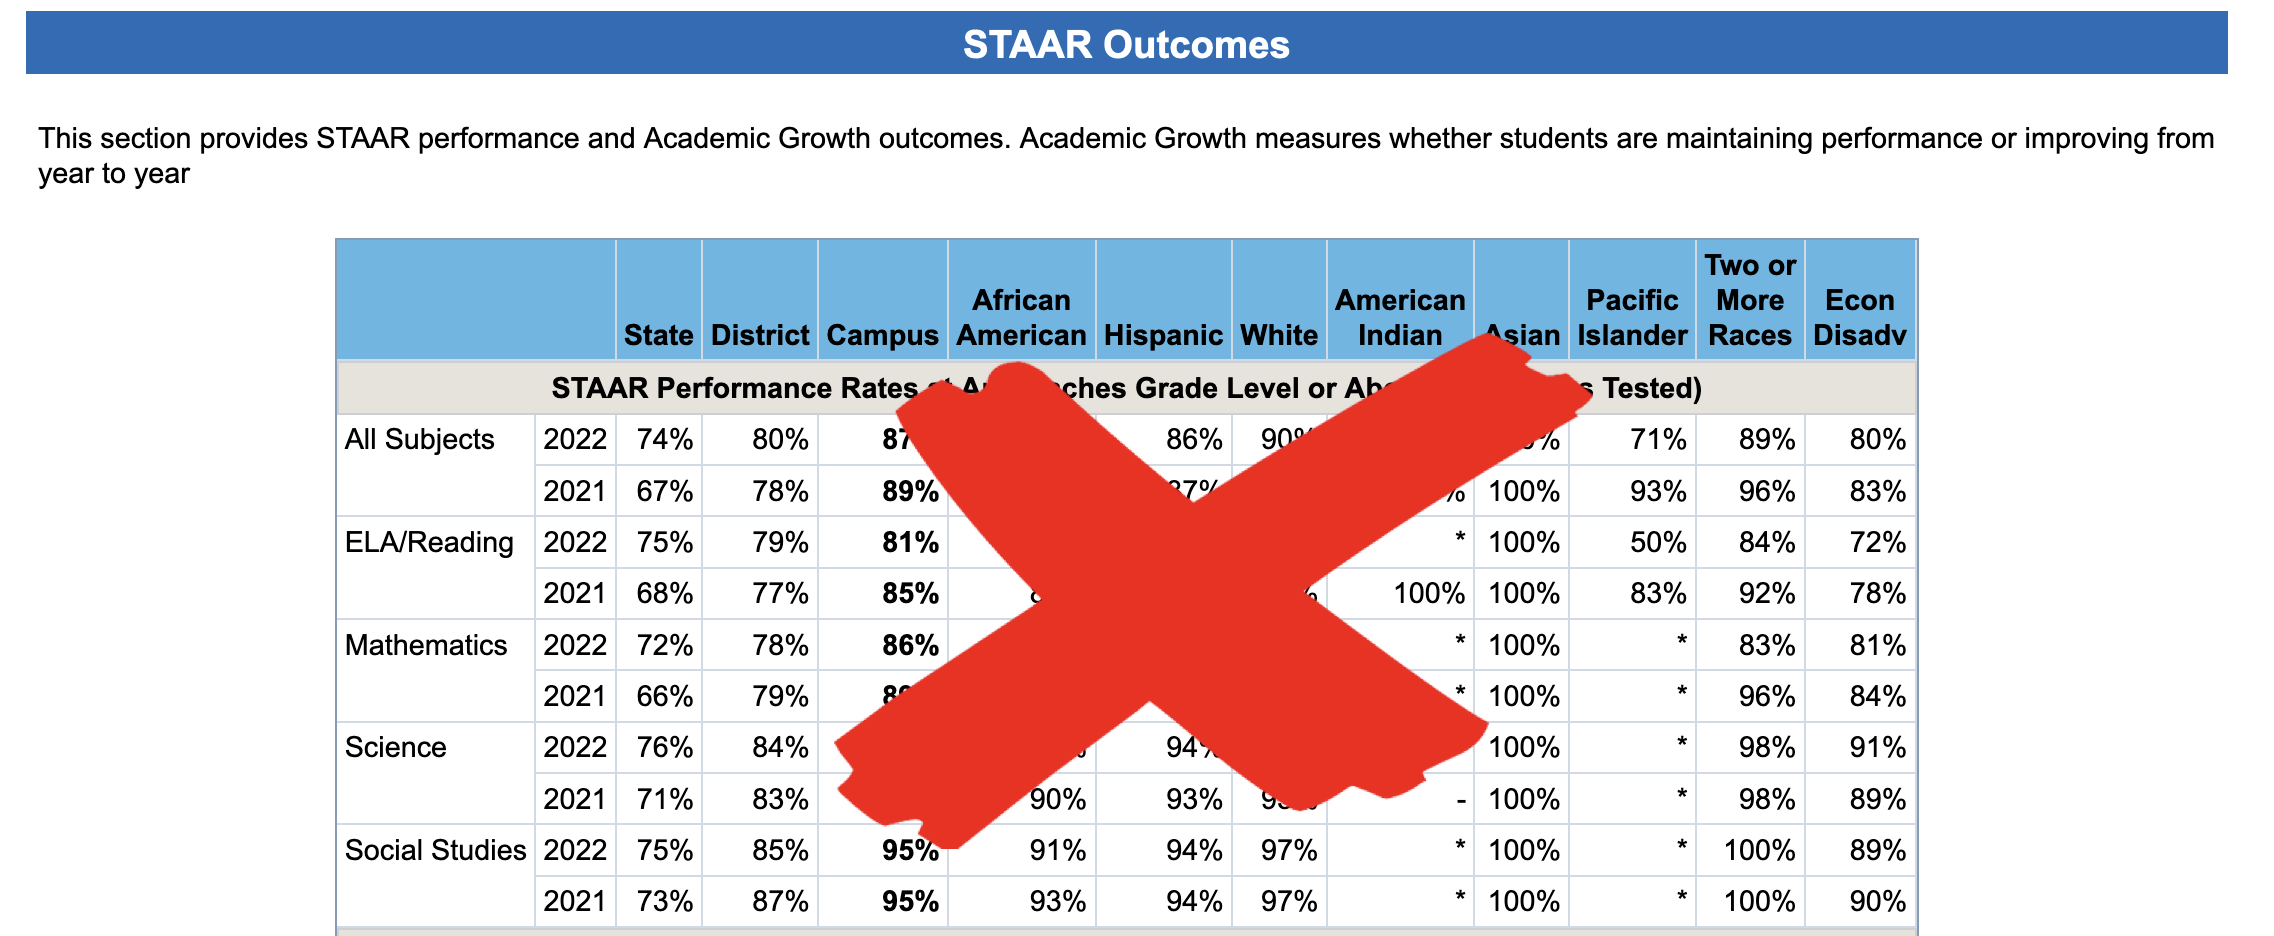
\includegraphics{img/crossed-out-staar-src-example-2021-2022-640-380.png}

Fig: This ``description-only'' form of report cannot help us to improve

\vspace{0.3in}

The crucial information for analysis of district output capability (and
the prediction of future performance) is contained in the order of
occurrence found in the time-period-by-time-period data.
\textbf{\emph{The more periods included in the analysis, the stronger
the evidence for your inferences from the charts.}}

Management in all forms is prediction. Therefore, management should
\textbf{\emph{use analytic reports}} instead of
\textbf{\emph{`description-only'}} reports. Management should focus on
improvement of processes for future results, not solely on judgment of
past results.



\end{document}
